\documentclass[12pt]{article}
\usepackage[russian]{babel}
\usepackage[utf8]{inputenc}
\usepackage{graphicx}
\usepackage{amsmath}
\usepackage{float}
\usepackage{geometry}
\usepackage{longtable}
\usepackage{enumitem}
\usepackage{listings}
\usepackage{xcolor}
\usepackage{indentfirst} % Для отступов в первом абзаце
\usepackage{subcaption} 
\usepackage[skip=5pt]{caption}
\usepackage{siunitx}
\usepackage{booktabs}
\usepackage{array}
\usepackage{hyperref}
\usepackage{setspace}

% Настройки русской типографии
\geometry{a4paper, left=30mm, right=15mm, top=20mm, bottom=20mm}
\setlength{\parindent}{1.25cm} % Красная строка
\setlength{\parskip}{0pt}      % Убираем отступы между абзацами
\linespread{1}               % Полуторный интервал

% Настройка гиперссылок
\hypersetup{
    colorlinks=true,
    linkcolor=blue,
    urlcolor=blue,
    citecolor=black,
}

% Стиль библиографии
\bibliographystyle{gost2015}

% Настройка листингов
\lstdefinelanguage{JavaScript}{
    keywords={let, const, function, return},
    sensitive=false,
    morecomment=[l]{//},
    morecomment=[s]{/*}{*/}
}

\lstset{
    basicstyle=\ttfamily\small,
    keywordstyle=\color{blue},
    commentstyle=\color{green},
    stringstyle=\color{red},
    numbers=left,
    numberstyle=\tiny\color{gray},
    frame=single,
    breaklines=true
}

% Настройка формата чисел
\sisetup{
    output-decimal-marker = {.},
    group-digits = false
}

\begin{document}

\tableofcontents

\newpage

\section{Введение}

В современном мире скорость загрузки веб-сайта играет критически важную роль для обеспечения положительного пользовательского опыта (User Experience, UX)
и достижения высоких позиций в результатах поиска. С ростом требований пользователей к быстродействию и доступности информации оптимизация скорости
загрузки сайтов стала неотъемлемой частью процесса разработки веб-приложений. Медленная загрузка страниц может привести к ухудшению показателей вовлечённости,
увеличению показателя отказов и, как следствие, снижению рейтинга сайта в поисковых системах.

Одним из способов увеличения скорости загрузки является применение сжатия для статических файлов, изображений и запросов.
При этом необходимо грамотно подбирать степень сжатия из-за накладных расходов на компрессию и декомпрессию.
В данной работе мы попытаемся определить \textbf{оптимальные} с определённой точки зрения параметры сжатия в зависимости от характеристик аппаратной части клиента и сервера,
а также пропускной способности сети.

Кроме того, сжатие позволяет снизить нагрузку на сеть и существенно сэкономить трафик.
Может показаться, что в современном мире высокоскоростного интернета на это уже не стоит обращать внимания.
Однако по состоянию на весну 2025 года Amazon (\url{https://aws.amazon.com/ru/cloudwatch/pricing/}) взимает
плату в размере 0{,}5~\text{\$} за 1~ГБ трафика, что для небольших IT-стартапов является существенной статьёй расхода.

На просторах интернета уже существует множество сравнений популярных методов сжатия, таких как Gzip и Brotli, JPEG и WebP:

\begin{itemize}
    \item Brotli и GZIP: \href{https://medium.com/@bansal.suneet/brotli-vs-gzip-compression-surprising-compression-result-brotli-power-782aac2ee29f}{Medium: Brotli и GZIP}
    \item Brotli и GZIP: \href{https://ddos-guard.ru/blog/algoritmy-brotli-recompressiya-i-HSTS-chto-novogo-predlagaet-DDoS-GUARD}{DDoS-Guard о Brotli}
    \item JPEG и WebP: \href{https://medium.com/@inna_netum/действительно-ли-webp-лучше-jpeg-91639d852035}{Сравнение WebP и JPEG}
\end{itemize}

Однако в большинстве случаев авторы ограничиваются такими параметрами, как степень сжатия, скорость компрессии и декомпрессии,
что трудно напрямую соотнести с ключевыми метриками, такими как LCP (Largest Contentful Paint — время до отрисовки самого большого элемента)
и RPS (Requests Per Second — число запросов в секунду).

Основная задача данной работы — определить и обосновать оптимальные параметры сжатия для загрузки и функционирования
веб-приложений в условиях изменяющейся сетевой нагрузки. В рамках исследования предполагается разработка системы,
способной адаптировать параметры сжатия в реальном времени для обеспечения бесперебойной работы и быстрого отклика приложений,
с учётом изменения числа пользователей и интенсивности их активности.

\section{Описание объекта исследования}

В ходе данной работы мы будем тестировать алгоритмы сжатия на примере REST API
(Representational State Transfer Application Programming Interface / программный интерфейс приложения для передачи репрезентативного состояния)
и SPA (Single Page Application / одностраничное веб-приложение) веб-приложения, выполняющего роль видеохостинга.
Сжатие видео в рамках данной работы не рассматривается.

Видеохостинг должен выполнять следующую бизнес-логику:

\begin{itemize}
    \item Аутентификация пользователей;
    \item Возможность добавления, удаления и просмотра видео;
    \item Формирование персональных рекомендаций;
    \item Возможность оставлять комментарии и ставить лайки под видео.
\end{itemize}

\subsection{Стек технологий}

\begin{figure}[H]
    \centering
    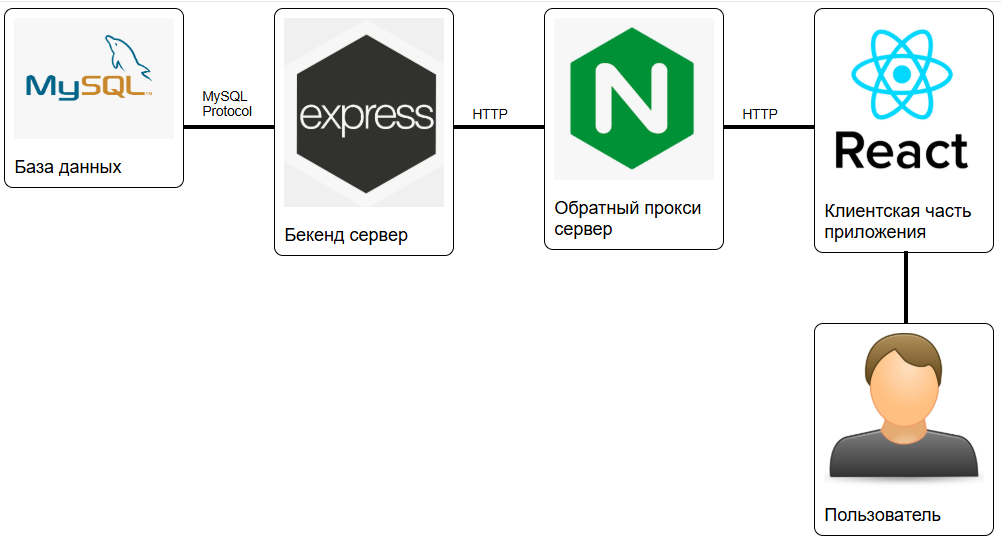
\includegraphics[width=1\textwidth]{../images/Схема_веб-приложения.png}
    \caption{Схема веб-приложения}
\end{figure}

Вкратце опишем, для чего нужен каждый элемент схемы:

\begin{itemize}
    \item \textbf{Backend} — сервер, обрабатывающий запросы от пользователя, отвечающий за аутентификацию и реализацию бизнес-логики.
          Например, подбор рекомендаций видео для конкретного пользователя, загрузка и удаление видео;

    \item \textbf{Frontend} — часть веб-приложения, работающая на стороне пользователя.
          Пользователь загружает статические файлы сайта, которые впоследствии исполняются в браузере.
          HTML отвечает за разметку, CSS — за стили, а JS обеспечивает функциональность и делает сайт интерактивным;

    \item \textbf{База данных} — необходима для удобного хранения большого объёма информации;

    \item \textbf{Обратный прокси-сервер} — выполняет вспомогательные операции с запросами.
          Помимо перенаправления, он может выполнять сжатие, кэширование, предоставление доступа к статическим файлам и балансировку нагрузки.
\end{itemize}

Используемый стек технологий:

\begin{itemize}
    \item Express.js — backend-сервер;
    \item React.js — frontend-часть приложения;
    \item MySQL — реляционная база данных;
    \item Nginx — обратный прокси-сервер.
\end{itemize}

\subsection{Характеристики аппаратной части сервера}

\begin{itemize}
    \item CPU: 1 vCPU;
    \item RAM: 2 GB;
    \item Storage: 20 GB;
    \item Network speed: 500 Mbps.
\end{itemize}

\subsection{Сценарий работы пользователя}

Пользователь переходит по ссылке или вводит в строку поиска \texttt{http://example-videohosting.ru}.
В этом случае на сервер передаётся HTTP GET-запрос, по которому возвращается файл \verb|index.html|.

Этот файл выглядит следующим образом:

\begin{lstlisting}[language=HTML]
<!DOCTYPE html>
<html lang="en">
<head>
    <meta charset="UTF-8">
    <meta name="viewport" content="width=device-width, initial-scale=1.0">
    <title>Videohosting</title>
    <link rel="stylesheet" href="./main.css">
    <script src="./main.js"></script>
</head>
<body>
    <img src="./assets/images/image.png">
    ...
</body>
</html>
\end{lstlisting}

После загрузки файла браузер начинает его обрабатывать:

\begin{itemize}
    \item Строится DOM (Document Object Model — представление HTML-документа в виде дерева элементов);
    \item Подгружаются CSS-файлы (строка 7);
    \item Загружаются и исполняются JS-файлы (строка 8);
    \item Загружаются и отрисовываются изображения (строка 11).
\end{itemize}

Когда этот процесс завершается, можно считать, что приложение полностью загружено и готово к использованию.

Далее пользователь может выполнять HTTP-запросы для отправки форм, загрузки данных с backend-сервера.

Исходя из вышесказанного, можно применять сжатие как для \textbf{статических данных} (файлов сайта), так и для \textbf{динамических данных}.
Дадим более подробные определения введённых понятий:

\begin{itemize}
    \item \textbf{Статические данные} — это данные, которые неизменны для каждого пользователя.
          К ним относятся HTML-, JS-, CSS-файлы сайта, а также изображения;

    \item \textbf{Динамические данные} — это данные, изменяющиеся во время работы приложения.
          К ним относится информация о видео (видео могут добавляться или удаляться, изменяется количество просмотров, отметок "нравится" и т. д.).
\end{itemize}

Мы отдельно рассмотрим сжатие статических и динамических данных.

Начнём с методов сжатия изображений.

\subsection{О форматах изображений}

Перед тем как приступить к описанию форматов, приведу критерии, по которым я буду их сравнивать:

\begin{itemize}
    \item \textbf{Степень сжатия} — отношение размеров исходного (в формате PNG) и сжатого изображений;
    \item \textbf{Скорость компрессии/декомпрессии} — как быстро сервер сжимает изображение и как быстро клиент его разархивирует и отрисовывает;
    \item \textbf{Совместимость с разными браузерами} — важный параметр,
          так как формат с низким уровнем совместимости не может использоваться в реальном приложении
          из-за риска потерять большую часть пользователей. Для оценки этого параметра
          я буду использовать данные с сайта \url{https://caniuse.com/}, являющегося де-факто авторитетным справочником
          по технологиям в браузерах.
\end{itemize}

\subsubsection{JPEG}

Filename extension: jpg, jpeg, jpe, jif, jfif, jfi\\
MIME type: image/jpeg

JPEG (Joint Photographic Experts Group) поддерживается всеми браузерами
и является одним из самых популярных форматов изображений.\\
Поддерживаются изображения с линейными размерами не более 65535 × 65536 пикселей.\\

Алгоритм JPEG наиболее эффективен для сжатия фотографий, содержащих реалистичные сцены
с плавными переходами яркости и цвета. Для хранения чертежей, текстовой и знаковой
графики лучше использовать PNG, GIF
или режим сжатия Lossless JPEG.

Уделим этому формату больше внимания, чем остальным, так как он зарекомендовал себя временем
и применяется гораздо чаще других. JPEG позволяет сжимать изображения как с потерями,
так и без потерь.
На его примере мы также постараемся понять, как можно регулировать степень сжатия.

При сжатии изображение преобразуется из цветового пространства $RGB$ в $YC_{b}C_{r}$.
Стандарт ISO/IEC 10918-1 не регламентирует выбор именно $YC_{b}C_{r}$,
допуская и другие варианты преобразования.

$Y$ — компонента яркости, $C_{B}$ и $C_{R}$ — сине- и красноцветоразностные компоненты.

Пространство $YC_{b}C_{r}$ выбрано не случайно: это связано с тем, что глаз человека гораздо лучше
различает яркость, чем цветовые оттенки, для которых выполняется прореживание.
В схеме прореживания 4:2:0 каждому блоку из 4 пикселей (2×2) ставится в соответствие
усреднённое значение $C_{B}$ и $C_{R}$.
Таким образом, вместо 12 значений (4×$Y$, 4×$C_{B}$, 4×$C_{R}$)
используется только 6 значений (4×$Y$, 1×$C_{B}$, 1×$C_{R}$).
Если к изображению предъявляются более высокие требования по качеству,
могут применяться схемы прореживания 4:4:0, 4:2:2 или вообще не применяться (4:4:4).

Стандарт допускает также прореживание блоков не 2×2, а 4×1 или 1×4,
но на практике такие схемы используются довольно редко.

После этого компоненты $Y$, $C_{B}$, $C_{R}$ разбиваются на блоки 8×8.
Каждый такой блок подвергается дискретному косинусному преобразованию (ДКП).

Формула для вычисления коэффициентов ДКП $F(u,v)$ блока 8×8:

\[
    F(u,v) = \frac{C(u)C(v)}{4} \sum_{x=0}^{7} \sum_{y=0}^{7} f(x,y) \cdot \cos\left(\frac{(2x+1)u\pi}{16}\right) \cos\left(\frac{(2y+1)v\pi}{16}\right)
\]

где:
\begin{itemize}
    \item $f(x,y)$ — значение пикселя в позиции $(x,y)$,
    \item $u,v$ — частотные координаты (от 0 до 7),
    \item $C(k)$ — нормировочный коэффициент:
          \[
              C(k) = \begin{cases}
                  \frac{1}{\sqrt{2}}, & \text{при } k=0, \\
                  1,                  & \text{иначе}.
              \end{cases}
          \]
\end{itemize}

Далее к полученной матрице применяется квантование (в зависимости от степени сжатия):

\[
    Q(u, v) = \text{round}\left(\frac{F(u, v)}{Q_{table}(u, v)}\right)
\]

После этого многие высокочастотные коэффициенты становятся равными нулю.

Полученные коэффициенты записываются в массив и кодируются с помощью кодов Хаффмана,
о которых будет рассказано в разделе <<2.4. О алгоритмах сжатия данных без потерь>>.

\subsubsection{PNG}

Filename extension: png\\
MIME type: image/png

PNG (Portable Network Graphics) — это растровый формат изображений, который обеспечивает сжатие
без потерь. Ещё одна особенность формата PNG — поддержка альфа-канала (прозрачности).

Согласно сайту \url{https://caniuse.com/}, весной 2025 года поддерживается 92{,}6\% браузеров.

\subsubsection{WebP}
Filename extension: webp\
MIME type: image/webp

WebP — это формат изображений, разработанный Google, который поддерживает сжатие изображений
с потерями и без потерь. Он призван обеспечить высокое качество изображений при меньших размерах файлов.\

Согласно сайту caniuse.com, поддерживается 95,92% браузеров весной 2025 года.

\subsubsection{AVIF}

AVIF (AV1 Image File Format) — современный формат изображений,
основанный на технологии сжатия AV1. Он предназначен для обеспечения высокого
качества изображений при более низком размере файлов.

Согласно сайту caniuse.com, поддерживается 93,71% браузеров весной 2025 года.

\subsubsection{HEIF/HEIC}
Filename extension: heif, heic\
MIME type: image/heif, image/heic\

HEIF (High Efficiency Image Format) — современный формат изображений,
обеспечивающий высокую эффективность сжатия и поддержку различных функций,
таких как анимация, HDR, прозрачность и многослойность.

HEIC (High Efficiency Image Container) — контейнерный формат файла,
используемый, в частности, для хранения изображений в формате HEIF.
Пример — Live Photos, сделанные на iPhone.

Согласно сайту caniuse.com, поддерживается 13,99% браузеров весной 2025 года,
только на устройствах Apple. По причине низкой совместимости в измерениях участвовать не будет.

\subsubsection{SVG}
Filename extension: svg\
MIME type: image/svg+xml

SVG (Scalable Vector Graphics) — формат изображений, основанный на XML,
который описывает двумерную векторную графику с использованием объектов,
таких как линии, кривые, формы и текст. Используется для логотипов и векторных изображений.
Для растровых изображений не подходит, поэтому в измерениях участвовать не будет.

Согласно сайту caniuse.com, поддерживается 96,99% браузеров весной 2025 года.

\subsection{Об алгоритмах сжатия данных без потерь}

\subsubsection{Алгоритм Хаффмана}

\textbf{Префиксный код} — это такой код, ни один символ которого не является префиксом другого.

Идея алгоритма состоит в том, что если известны вероятности появления символов,
можно построить оптимальные префиксные коды. Оптимальность
означает, что $H \leq L \leq H + 1$, где $L$ — средняя длина кода на символ, $H$ — энтропия.
Символам с наибольшей вероятностью соответствуют более короткие коды.

Алгоритм на входе получает таблицу частотностей символов в сообщении.
Затем на основании этой таблицы строится дерево кодирования Хаффмана.

На данный момент браузерами поддерживаются два основных алгоритма сжатия без потерь,
применяемых для текстовых файлов (CSS, HTML, JS):

\begin{itemize}
    \item Gzip
    \item Brotli
\end{itemize}

Прежде чем приступить к описанию этих алгоритмов, следует рассказать
о семействе алгоритмов LZ, в частности LZ77, так как оба основаны на нём.
Алгоритмы словарного сжатия Зива — Лемпела появились во второй половине 1970-х годов.
Это были алгоритмы LZ77 и LZ78, разработанные совместно
Зивом (Ziv) и Лемпелом (Lempel). В дальнейшем они подверглись множественным
модификациям, и сегодня существует десятки самостоятельных алгоритмов
и бесчисленное множество их версий.

LZ77 и LZ78 являются универсальными алгоритмами сжатия,
в которых словарь формируется на основании уже обработанной части входного потока,
т. е. адаптивно. Основное отличие между ними — в способе формирования фраз.

\subsubsection{Алгоритм LZ77}

Алгоритм LZ77 — родоначальник целого семейства словарных схем,
так называемых алгоритмов со скользящим словарём (или окном).
В LZ77 в качестве словаря используется блок уже закодированной последовательности.
Как правило, по мере обработки положение этого блока относительно начала
последовательности изменяется — словарь "скользит" по входному потоку данных.

Скользящее окно имеет длину $N$, т. е. в него помещается $N$ символов, и состоит из двух частей:

\begin{itemize}
    \item Последовательности длиной $W = N - n$ уже закодированных символов, которая и является словарём;
    \item Упреждающего буфера (буфера предварительного просмотра) длиной $n$; обычно $n$ на порядок меньше $W$.
\end{itemize}

Пусть к текущему моменту времени мы уже закодировали $t$ символов, последние $W$ символов будут
составлять словарь. На каждой итерации алгоритма ищется самое длинное вхождение префикса
строки упреждающего буфера (начиная с символа $t+1$) в словаре + буфере,
причём часть строки обязательно должна находиться в словаре. Полученная фраза
кодируется с помощью двух чисел:

\begin{enumerate}
    \item Смещение (offset) от начала буфера;
    \item Длина совпадения (match length).
          Смещение и длина совпадения однозначно указывают на фразу.
          Дополнительно в выходной поток записывается символ $s$,
          непосредственно следующий за совпавшей строкой буфера.
\end{enumerate}

Декодирование сжатых данных осуществляется путём простой
замены кода на блок символов, состоящий из фразы из словаря и передаваемого символа.
Декодер должен выполнять те же действия по изменению окна, что и кодер.
Фраза словаря легко восстанавливается по смещению и длине,
поэтому важным свойством LZ77 и подобных алгоритмов со скользящим окном является
высокая скорость декодирования.

Алгоритмы со скользящим окном характеризуются сильной несимметричностью по времени:
кодирование значительно медленнее декодирования,
так как при сжатии много времени уходит на поиск фраз.

\subsubsection{Формат Deflate}

Формат словарного сжатия Deflate, предложенный Катцем (Katz),
используется в популярном архиваторе GZIP.
Сжатие осуществляется с помощью алгоритма типа LZH —
иначе говоря, указатели и литералы кодируются по методу Хаффмана.
Формат специфицирует только работу декодера, т. е. определяет алгоритм декодирования
и не налагает серьёзных ограничений на реализацию кодера.

В принципе, в качестве алгоритма сжатия может применяться любой, работающий со скользящим окном,
при условии, что он использует стандартную процедуру обновления словаря для алгоритмов семейства LZ77
и применяет задаваемые форматом типы кодов Хаффмана.

Закодированные в соответствии с форматом Deflate данные представляют собой набор блоков,
порядок которых совпадает с последовательностью соответствующих блоков исходных данных.
Используются три типа блоков закодированных данных:

\begin{enumerate}
    \item Состоящие из несжатых данных;
    \item Использующие фиксированные коды Хаффмана;
    \item Использующие динамические коды Хаффмана.
\end{enumerate}

Длина блоков первого типа не может превышать 64 КБ; других ограничений по размеру не установлено.
Каждый блок второго и третьего типов состоит из двух частей:

\begin{itemize}[label=-]
    \item описания двух таблиц кодов Хаффмана, используемых для кодирования данных блока;
    \item собственно закодированных данных.
\end{itemize}

Коды Хаффмана в каждом блоке не зависят от кодов, использованных в предыдущих блоках.
Сама структура динамически создаваемых кодов Хаффмана также сжимается с помощью фиксированных кодов Хаффмана,
таблица которых задаётся форматом.

Алгоритм словарного сжатия может использовать в качестве словаря часть предыдущего блока (или блоков),
но смещение не может превышать 32 КБ.

Данные в компактном представлении состоят из кодов элементов двух типов:

\begin{itemize}[label=-]
    \item литералов (отдельных символов);
    \item указателей на имеющиеся во входном потоке фразы; указатели состоят из пары
          <длина совпадения, смещение>.
\end{itemize}

Длина совпавшей строки не может превышать 258 байт, а смещение фразы — 32 КБ.
Литералы и длины совпадения кодируются с помощью одной таблицы кодов Хаффмана,
а для смещений используется другая таблица.
Иначе говоря, литералы и длины совпадения образуют один алфавит.
Именно эти таблицы кодов и передаются в начале блока третьего типа.

\subsubsection{Формат сжатия Gzip (GNU zip)}

Это утилита для сжатия и распаковки файлов, широко используемая в UNIX-системах.
Формат файла Gzip состоит из трёх основных частей:

\begin{enumerate}
    \item Заголовок: содержит информацию о типе файла, имени оригинального файла, времени создания, уровне сжатия и других параметрах.
    \item Тело: содержит сжатые данные, полученные с помощью алгоритма DEFLATE.
    \item Контрольная сумма (CRC-32) и размер оригинала: эти данные позволяют проверить целостность и корректность распаковки.
\end{enumerate}

Заголовок файла содержит следующие ключевые поля:

\begin{itemize}[label=-]
    \item ID1 и ID2: идентификаторы, указывающие на формат Gzip (значения — 0x1F и 0x8B);
    \item CM: метод сжатия (в Gzip используется значение 8 для DEFLATE);
    \item FLG: биты флагов, указывающие на наличие дополнительных полей и информации;
    \item MTIME: время последней модификации оригинального файла;
    \item XFL: дополнительная информация о методе компрессии;
    \item OS: платформа, на которой был создан/сжат файл (Gzip).
\end{itemize}

Теоретически возможны и другие значения для поля метода сжатия,
но сам формат Gzip и его стандартная реализация предполагают использование только DEFLATE.
На практике, если файл Gzip содержит метод сжатия, отличный от DEFLATE,
стандартные утилиты для работы с файлами Gzip могут его не поддерживать и не распознать.

\subsubsection{За счёт чего можно добиться разных степеней сжатия?}

Поскольку формат Deflate не имеет чёткой спецификации алгоритма словарного сжатия,
разработчики могут использовать различные модификации LZH, подбирая параметры
для обеспечения желаемого соотношения скорости и коэффициента сжатия.
В качестве одного из вариантов можно, например, ограничить длину совпадающей последовательности.

\subsection{Инструменты разработчика браузера}

\subsubsection{Браузеры и JavaScript}

На сегодняшний день существует два основных вида браузеров:

\begin{itemize}[label=-]
    \item Основанные на движке Chromium V8 от Google (https://github.com/v8/v8), такие как
          Google Chrome, Yandex Browser, Microsoft Edge и другие;
    \item Firefox, использующий движок Quantum.
\end{itemize}

JavaScript, применяемый в веб-приложениях, является скриптовым языком.
Существует спецификация ECMAScript (https://262.ecma-international.org/),
в которой описано, что должен делать язык, но не указано, как это реализуется.
Реализация функций языка ложится на плечи разработчиков браузеров.

В отличие от C или Java, в экосистеме JavaScript нет универсального компилятора
или виртуальной машины (например, JVM).
Разработчики веб-приложений зачастую не знают точно, что происходит "под капотом".

Для получения информации о времени выполнения, скорости загрузки,
использовании памяти и других характеристиках можно использовать инструменты разработчика (DevTools).
Их можно открыть в любом браузере, нажав клавишу F12.

\subsubsection{Какие функции предоставляет консоль разработчика}

Реализация DevTools может отличаться в зависимости от браузера,
но в целом интерфейс у браузеров на базе Chromium весьма схож.
В качестве примера далее будет использоваться Google Chrome.

Особый интерес представляют две вкладки:

\subsubsection{Network}

\begin{figure}[H]
    \centering
    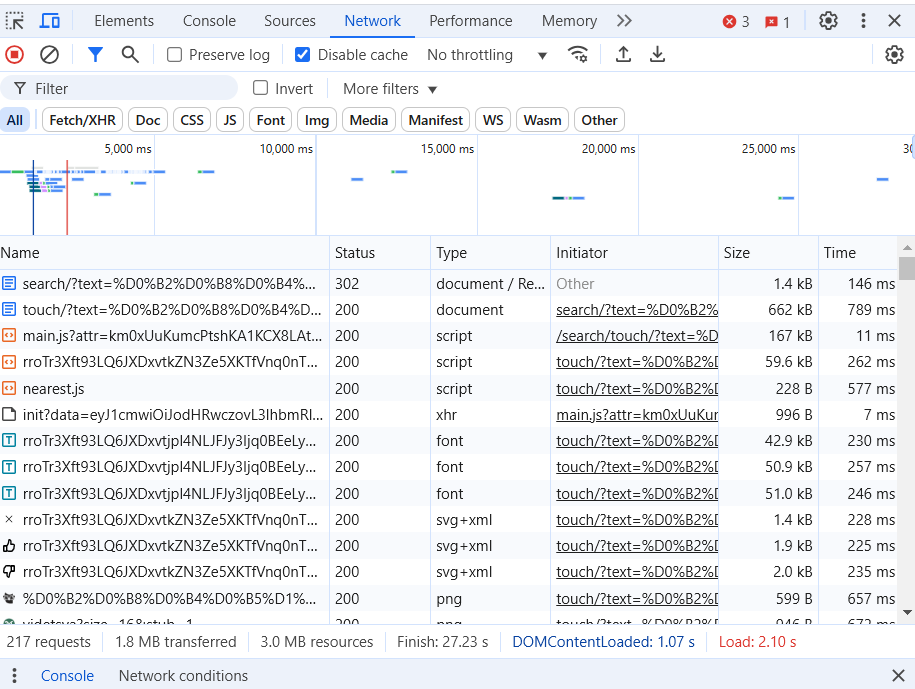
\includegraphics[width=1\textwidth]{../images/network.png}
    \caption{Вкладка Network}
\end{figure}

На этой вкладке можно просматривать все сетевые запросы, выполненные браузером при загрузке страницы:
узнать статус запроса, его тип, размер ответа и общее время, затраченное на HTTP-запрос.

Если нажать на конкретный запрос, можно будет увидеть такие временные интервалы, как:

\begin{itemize}[label=-]
    \item Время отправки запроса (отсчитывается с момента перехода на сайт);
    \item Queueing (Очередь) — браузер ставит запросы в очередь перед началом соединения, если:
          - существуют запросы с более высоким приоритетом (приоритет зависит от типа ресурса и его позиции в документе);
          - для данного источника уже открыто шесть TCP-соединений, что является пределом для HTTP/1.0 и HTTP/1.1;
          - браузер кратковременно выделяет место в дисковом кеше;
    \item Stalled — запрос мог быть приостановлен после начала соединения по любой из вышеуказанных причин;
    \item Initial connection — время, затраченное на TLS/SSL handshake (если используется HTTPS) и на TCP handshake;
    \item Request sent — время, затраченное на отправку запроса;
    \item Waiting (TTFB) — время ожидания ответа от сервера (Time to First Byte);
    \item Content download — время, затраченное на загрузку тела ответа.
\end{itemize}

\begin{figure}[H]
    \centering
    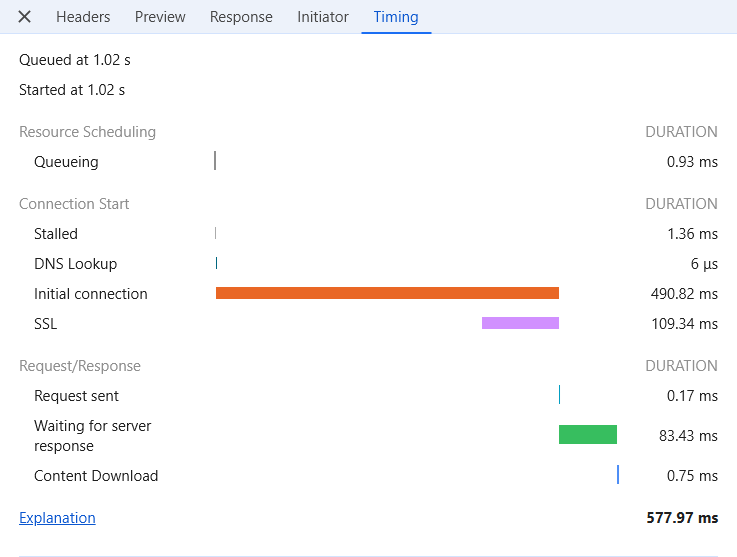
\includegraphics[width=1\textwidth]{../images/network__timing.png}
    \caption{Временные интервалы конкретного запроса}
\end{figure}

Суммарное время запроса складывается из всех перечисленных этапов.
Как видно, по этим данным невозможно определить время,
затраченное на декодирование ответа.

\textbf{Немного о HTTP}

Считаю уместным сказать несколько слов о протоколе HTTP, чтобы иметь лучшее представление
о том, как с технической точки зрения применяется сжатие.
Первым делом браузер осуществляет HTTP-запрос, прикрепляя заголовок \textbf{Accept-Encoding}.
Современные браузеры поддерживают Gzip, Deflate, Brotli и Zstandard,
и заголовок может выглядеть следующим образом:
\textbf{Accept-Encoding: gzip, deflate, br, zstd}.

Сервер обрабатывает запрос, применяя к телу HTTP-ответа один из алгоритмов,
указанных в \textbf{Accept-Encoding}. В ответе сервер добавляет заголовок \textbf{Content-Encoding},
например, \textbf{Content-Encoding: br}, указывающий на применённый алгоритм.
Получив ответ, браузер может продолжить загрузку тела HTTP-ответа.

\subsubsection{Performance}

\begin{figure}[H]
    \centering
    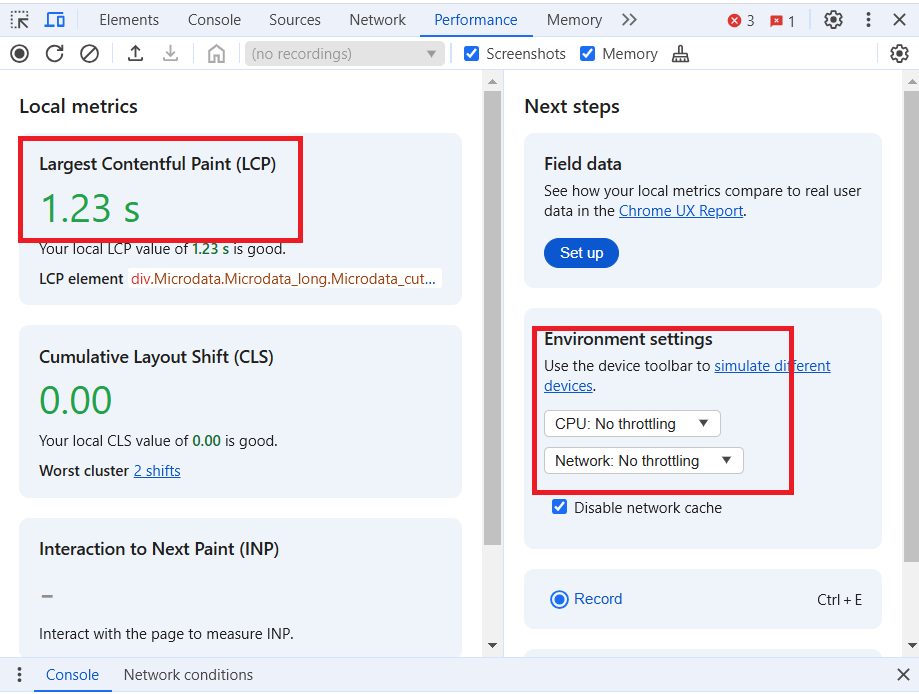
\includegraphics[width=1\textwidth]{../images/performance.png}
    \caption{Вкладка Performance}
\end{figure}

На этой вкладке также можно задать замедление для процессора или сети.

Largest Contentful Paint (LCP) (источник)
сообщает о времени рендеринга самого большого изображения, текстового блока или видео,
видимого в окне просмотра, относительно момента, когда пользователь впервые перешёл на страницу.
Браузер измеряет это время как момент, когда будет построено DOM-дерево,
выполнится JavaScript-код, применятся CSS-стили, загрузятся и отрисуются изображения.

Считается, что этот показатель используется поисковыми системами для ранжирования сайтов:
чем ниже $T_{LCP}$, тем выше сайт в поисковой выдаче.
Поэтому я буду уделять особое внимание LCP.

Для сети предусмотрено несколько предустановленных режимов. Например:

\begin{enumerate}
    \item Low-end Mobile (регламентировано для 3G):
          \begin{itemize}[label=-]
              \item Скорость загрузки (Download): 400 Кбит/с;
              \item Скорость отправки (Upload): 400 Кбит/с;
              \item Задержка (Latency): ~400 мс.
          \end{itemize}

    \item Regular 3G:
          \begin{itemize}[label=-]
              \item Скорость загрузки (Download): 750 Кбит/с;
              \item Скорость отправки (Upload): 250 Кбит/с;
              \item Задержка (Latency): ~100 мс.
          \end{itemize}

    \item Good 3G:
          \begin{itemize}[label=-]
              \item Скорость загрузки (Download): 1.5 Мбит/с;
              \item Скорость отправки (Upload): 750 Кбит/с;
              \item Задержка (Latency): ~40 мс.
          \end{itemize}
\end{enumerate}

Также можно задать собственную конфигурацию сети.

\subsubsection{Замедление процессора}

CPU-throttling в DevTools используется для замедления работы процессора
в целях эмуляции менее мощных устройств или реальных условий использования.
Это особенно полезно при тестировании производительности, чтобы понять,
как сайт или приложение будет работать на слабых устройствах,
например, на смартфонах, или в условиях высокой нагрузки.

На основании личного опыта могу предположить, что замедление в DevTools реализовано программно.
Браузер замедляет выполнение базовых функций JavaScript (таких как sort, map, for)
в заданное количество раз: 4x, 6x, 20x и т.д.
Исходя из этого, можно предположить, что замедление CPU не повлияет на время,
затраченное на декодирование файлов.

Также можно определить, какое замедление процессора требуется для эмуляции мобильных устройств.
На моём компьютере это оказалось примерно 2x (для смартфонов среднего сегмента)
и 6x (для устройств начального уровня).

\section{Измерения и анализ полученных результатов}

В этом разделе мы проведём серию экспериментов, используя различные методы сжатия,
и замерим ключевые показатели, такие как LCP и RPS (количество запросов в секунду),
чтобы выработать рекомендации по практическому применению.

Начнём с изображений и методов сжатия с потерями.

\subsection{Сравнение форматов изображений}

Изначально все изображения представлены в формате PNG.

Конвертация из PNG в JPEG с качеством 0.8 (обеспечивающим баланс между качеством
и степенью сжатия), в WebP — с помощью сайта https://image.online-convert.com/convert/,
в AVIF — на сайте https://converter.app/png-to-avif,
в HEIC — на сайте https://png2heic.com/.

Были выбраны 10 различных изображений (людей, природы, котов)
в формате PNG и сконвертированы в форматы JPEG, WebP, AVIF и HEIC.

\begin{figure}[H]
    \centering
    \begin{minipage}{0.48\textwidth}
        \centering
        
\includegraphics[width=\linewidth]{../images/image_comp/image1.png}
        \caption{Первое изображение}
        \label{fig:image1}
    \end{minipage}
    \hfill
    \begin{minipage}{0.48\textwidth}
        \centering
        
\includegraphics[width=\linewidth]{../images/image_comp/image4.png}
        \caption{Второе изображение}
        \label{fig:image2}
    \end{minipage}
\end{figure}

Размер 10 изображений в разных форматах:

\begin{itemize}[label=-]
    \item PNG: 18,0 МБ
    \item JPEG: 1,66 МБ
    \item WebP: 1,42 МБ
    \item AVIF: 1,00 МБ
    \item HEIC: 1,04 МБ
\end{itemize}

\subsubsection{Измерение времени декодирования}

Я начал с попытки получить информацию о времени декодирования напрямую
в DevTools. Для формата JPEG получилась следующая картина:

\begin{figure}[H]
    \centering
    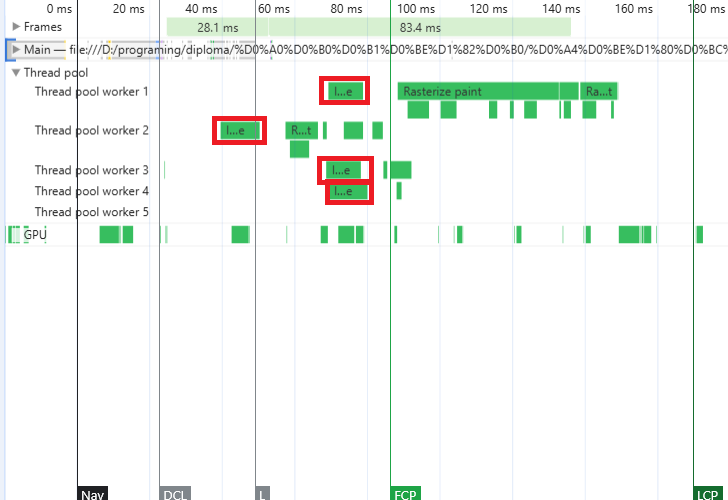
\includegraphics[width=1\textwidth]{../images/image_comp/devtools.png}
    \caption{Диаграмма загрузки потоков}
\end{figure}

Красными прямоугольниками выделено время декодирования изображений.

На данной диаграмме показаны временные интервалы, соответствующие декодированию и растеризации изображений.
По оси X отложено время в миллисекундах, по оси Y — задействованные потоки процессора.

Как видно, браузер умеет декодировать изображения параллельно.

В основном реализуется следующая схема:

\begin{enumerate}
    \item Браузер скачивает файл;
    \item Декодирует его;
    \item Отрисовывает.
\end{enumerate}

Однако, так как JPEG поддерживает последовательное декодирование,
может происходить следующее: браузер сначала декодирует часть изображения,
растеризует её, затем декодирует следующую часть и так далее.
На практике я наблюдал разбиение изображения на три части.

Для изображения размером 344 кБ было получено время декодирования
$T_{dec} = 13,4 \pm 1$ мс и время растеризации — $T_{ras} = 8,9 \pm 0,9$ мс.

С другими форматами ситуация обстоит хуже — браузер не предоставляет информации
о времени декодирования.

\begin{figure}[H]
    \centering
    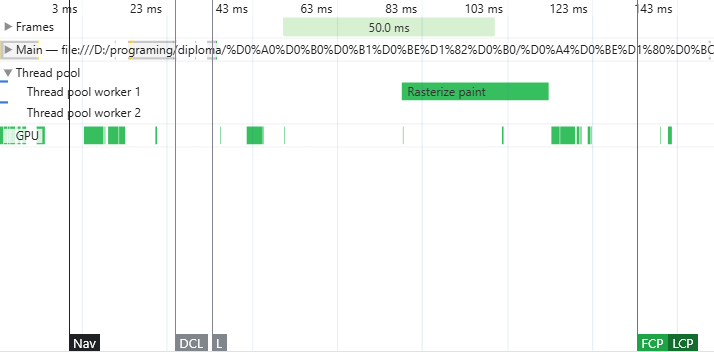
\includegraphics[width=1\textwidth]{../images/image_comp/avif_one_image.png}
    \caption{Диаграмма для AVIF}
\end{figure}

Время растеризации для AVIF составило $T_{ras} = 34,9 \pm 3,2$ мс,
что заметно хуже, чем у JPEG.

Мы можем измерить время, потраченное на декодирование + растеризацию косвенно.
Логично предположить, что $T_{LCP}$ измеряется по следующей формуле:

\[
    T_{LCP} = T_{\text{проч}} + T_{down} + T_{dec+ras}
\]

где:

\begin{itemize}
    \item $T_{\text{проч}}$ - время на рендеринг DOM, время на отправку
          запроса HTTP и прочие
          функции браузера, которые не зависят от формата;
    \item $T_{dec+ras}$ - время на декодирование и растеризацию;
    \item $T_{down}$ - время на загрузку файла: для JPEG $T_{down} = 1{,}3 \pm 0{,}2 \text{ мс}$,
          для PNG $T_{down} = 2{,}4 \pm 0{,}3 \text{ мс}$. Так как оно на порядок меньше $T_{dec+ras}$,
          им можно пренебречь.
\end{itemize}

Тогда, замерив $T_{LCP}$ для разных форматов, можно найти разность $T_{dec+ras}$.

\begin{table}[H]
    \centering
    \caption{Результаты измерений LCP}
    \begin{tabular}{l S[table-format=3.1] S[table-format=2.2]}
        \toprule
        Формат & {$\overline{T}_{\text{LCP}}$, \text{мс}} & {$\sigma$, \text{мс}} \\
        \midrule
        JPEG   & 73                                       & 8                     \\
        PNG    & 141                                      & 7                     \\
        AVIF   & 139                                      & 6                     \\
        WebP   & 125                                      & 6                     \\
        \bottomrule
    \end{tabular}
\end{table}

Считая, что для JPEG $T_{dec+ras} = 22{,}8 \pm 2 \text{ мс}$, получим:

\begin{table}[H]
    \centering
    \caption{Время декодирования и растеризации}
    \begin{tabular}{l S[table-format=2.1] S[table-format=1.2]}
        \toprule
        Формат & {$\overline{T}_{dec+ras}$, \text{мс}} & {$\sigma$, \text{мс}} \\
        \midrule
        JPEG   & 22                                    & 2                     \\
        PNG    & 90                                    & 9                     \\
        AVIF   & 88                                    & 8                     \\
        WebP   & 74                                    & 8                     \\
        \bottomrule
    \end{tabular}
\end{table}

Попробуем определить критерии оптимального формата с точки зрения LCP.
Предположим, у нас есть некоторое изображение.
Также у нас постоянные характеристики аппаратной части клиента.
Тогда $T_{LCP}$ зависит только от двух параметров: $V_{down}$ и $i_{comp}$, где:

\begin{itemize}
    \item $V_{down}$ - скорость загрузки пользователя;
    \item $i_{comp}$ - формат кодирования.
\end{itemize}

Тогда:

\[
    T_{LCP} = T_{LCP}(V_{down}, i_{comp}) = T^{i}_{\text{проч}} + T^{i}_{down} + T^{i}_{dec+ras} = T_{\text{проч}} + \frac{M_{\text{исх}}}{k_{i} \cdot V_{down}} + T^{i}_{dec+ras}
\]

$M_{\text{исх}}$ - исходный вес изображения в Мб; \\
$k_i$ - степень сжатия. \\

Используя эту формулу, найдём скорость загрузки пользователя, при которой $T^{JPEG}_{LCP} = T^{AVIF}_{LCP}$ для протестированного изображения:

\[
    T_{\text{проч}} + \frac{M_{\text{исх}}}{k_{JPEG} \cdot V^{equal}_{down}} + T^{JPEG}_{dec+ras} = T_{\text{проч}} + \frac{M_{\text{исх}}}{k_{AVIF} \cdot V^{equal}_{down}} + T^{AVIF}_{dec+ras}
\]

\begin{equation}
    V^{equal}_{down} = \frac{M_{\text{исх}}(k_{AVIF} - k_{JPEG})}{k_{JPEG}k_{AVIF}(T^{AVIF}_{dec+ras} - T^{JPEG}_{dec+ras})}
\end{equation}

$M_{\text{исх}} = 2{,}9\text{ Мб}$, $k_{JPEG} = 8{,}89$, $k_{AVIF} = 16{,}14$.

\[
    V^{equal}_{down} = 17{,}76 \text{ мбит/c}
\]

Что вдвое быстрее скорости загрузки хорошего 4G.
Выше этой скорости будет эффективнее JPEG, ниже - AVIF.

Чтобы проверить теоретические расчёты, предлагаю сравнить $T_{LCP}$ у JPEG
и AVIF для разных скоростей:

\begin{itemize}
    \item Fast 4G 7{,}5 мбит/c;
    \item «Double» 4G 18 мбит/c;
    \item Без замедления.
\end{itemize}

\begin{table}[H]
    \centering
    \caption{Сравнение LCP для разных скоростей}
    \begin{tabular}{l S[table-format=3.2] S[table-format=2.2]}
        \toprule
        Формат               & {$\overline{\text{LCP}}$, \si{\milli\second}} & {$\sigma$, \si{\milli\second}} \\
        \midrule
        Fast 4G, JPEG        & 799                                           & 20                             \\
        Fast 4G, AVIF        & 736                                           & 13                             \\
        «Double» 4G, JPEG    & 689                                           & 23                             \\
        «Double» 4G, AVIF    & 689                                           & 15                             \\
        Без замедления, JPEG & 151                                           & 5                              \\
        Без замедления, AVIF & 198                                           & 25                             \\
        \bottomrule
    \end{tabular}
\end{table}

Измерения подтверждают выведенную формулу. Может возникнуть вопрос: почему в этом измерении без замедления $LCP$ оказался больше, чем в предыдущем опыте?
Дело в сервере раздачи статических файлов, который позволил конфигурировать параметры сети.

Также стоит подметить, что LCP увеличился в случаях 4G и Double 4G из-за искусственной задержки ответа сервера,
что эмулирует реальную 4G-сеть.

\subsubsection{Практические рекомендации}

Учитывая, что полученная $V^{equal}_{down} = 17{,}76 \text{ мбит/c}$ соответствует пограничной скорости мобильного интернета,
следует использовать формат AVIF, если целевая аудитория сайта — пользователи мобильных устройств,
и JPEG — если используются десктопные устройства (100 мбит/c). Конечно, это справедливо только для случаев,
когда не требуется поддержка прозрачности. В противном случае рекомендуется использовать WebP.

\subsubsection{Случай с множеством изображений}

Когда на сайте несколько изображений, следует учитывать возможность параллельного декодирования и растеризации.
В этом случае $V^{equal}_{down}$ будет другой. Формула расчёта зависит от числа потоков, задействованных браузером.
В целом для нескольких изображений и многопоточных устройств из-за возможности параллельно декодировать
и отрисовывать изображения $V^{equal}_{down}$ оказывается в несколько раз выше.

\subsection{Сжатие статических файлов браузера с помощью Gzip и Brotli}

Приступим к измерению показателей методов сжатия без потерь. Но перед этим хочу акцентировать внимание на
формуле для вычисления полного времени скачивания сжатых данных:

\begin{equation}
    T_{\text{полн}} = T_{\text{comp}} + T_{down} + T_{decomp}
\end{equation}

где:
\begin{itemize}
    \item $T_{\text{comp}}$ — время сжатия данных (для статических файлов $T_{\text{comp}} = 0$);
    \item $T_{down}$ — время скачивания сжатого тела запроса (зависит от степени сжатия);
    \item $T_{decomp}$ — время декомпрессии.
\end{itemize}

\subsubsection{Что измеряем}

Для алгоритмов Gzip и Brotli будут измерены:
\begin{itemize}[label=-]
    \item степень сжатия;
    \item время сжатия;
    \item время декомпрессии.
\end{itemize}

В качестве исходных данных использованы минифицированные версии трёх веб-приложений:
\begin{itemize}[label=-]
    \item Dating App (DA);
    \item Videohosting (VH);
    \item Angular Conduit (AC).
\end{itemize}

\subsubsection{Технические характеристики устройства}

Процессор: Intel(R) Core(TM) i5-10210U CPU @ 1.60 ГГц, 2.11 ГГц\\
Оперативная память: 8,00 ГБ\\
Операционная система: Windows 11, версия 24H2, WSL Linux Ubuntu 20.04

\subsubsection{Условия проведения эксперимента и обработка данных}

Для сжатия методами Gzip и Brotli использована утилита gzipper на Node.js.

Для декомпрессии использованы утилиты gunzip и brotli на Linux.

Для замеров времени декомпрессии использован hyperfine.

Построены минимумы по времени.

Для точности измерений были отключены фоновые процессы операционной системы.

В веб-приложениях удалены файлы с изображениями, так как они уже сжаты с помощью специальных алгоритмов для изображений (JPG, WebP, AVIF).

Исходный размер приложений:
\begin{itemize}
    \item Dating App (DA) — 999 КБ;
    \item Videohosting (VH) — 479 КБ;
    \item Angular Conduit (AC) — 456 КБ.
\end{itemize}

\subsubsection{Измерение степени сжатия}

\begin{figure}[H]
    \centering
    \begin{minipage}{0.48\textwidth}
        \centering
        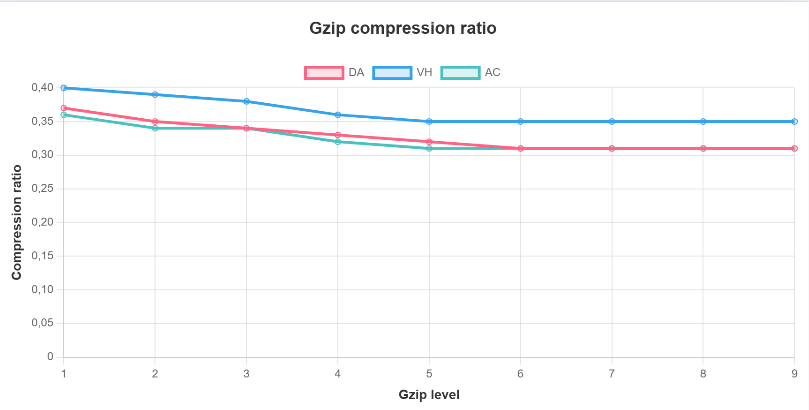
\includegraphics[width=\linewidth]{../images/gzip_compress_ratio.png}
        \caption{Степень сжатия Gzip}
        \label{fig:image1}
    \end{minipage}
    \hfill
    \begin{minipage}{0.48\textwidth}
        \centering
        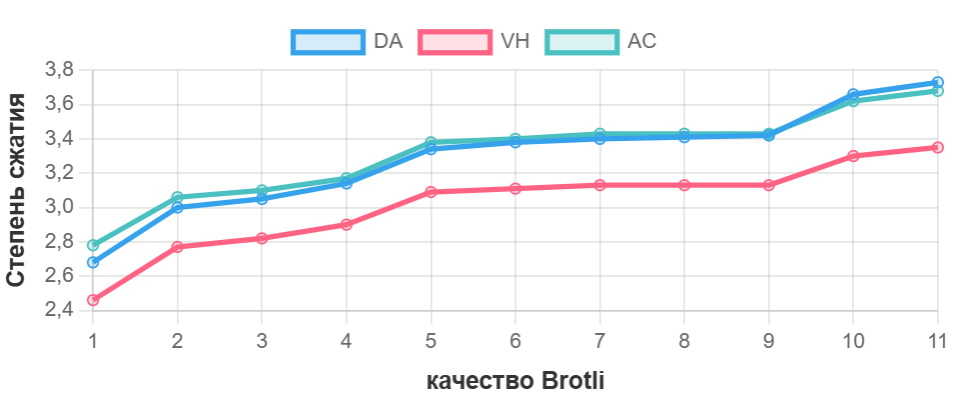
\includegraphics[width=\linewidth]{../images/brotli_compressed_ratio.png}
        \caption{Степень сжатия Brotli}
        \label{fig:image2}
    \end{minipage}
\end{figure}

\subsubsection{Измерение времени сжатия}

\begin{figure}[H]
    \centering
    \begin{minipage}{0.48\textwidth}
        \centering
        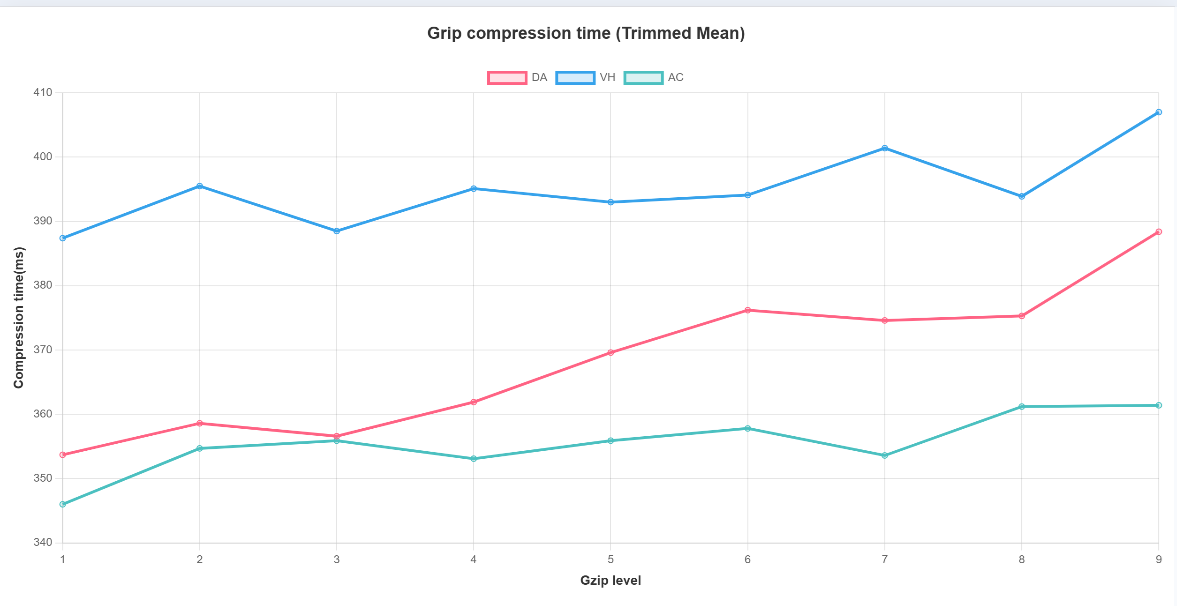
\includegraphics[width=\linewidth]{../images/Gzip compression time (Trimmed Mean).png}
        \caption{Время сжатия Gzip}
        \label{fig:image1}
    \end{minipage}
    \hfill
    \begin{minipage}{0.48\textwidth}
        \centering
        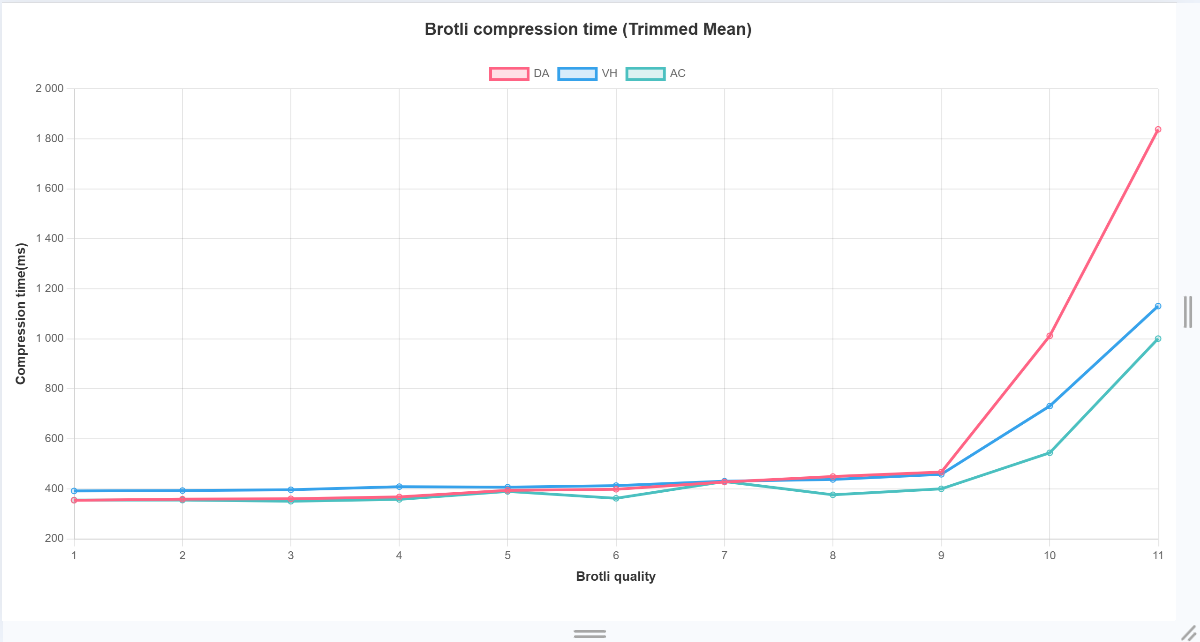
\includegraphics[width=\linewidth]{../images/Brotli compression time (Trimmed Mean).png}
        \caption{Время сжатия Brotli}
        \label{fig:image2}
    \end{minipage}
\end{figure}

Было замечено, что gzipper тратит 160 мс на пустой файл. Вероятно,
это время требуется для запуска процесса и выделения памяти. Поэтому также построены графики за вычетом времени на накладные расходы.

\begin{figure}[H]
    \centering
    \begin{minipage}{0.48\textwidth}
        \centering
        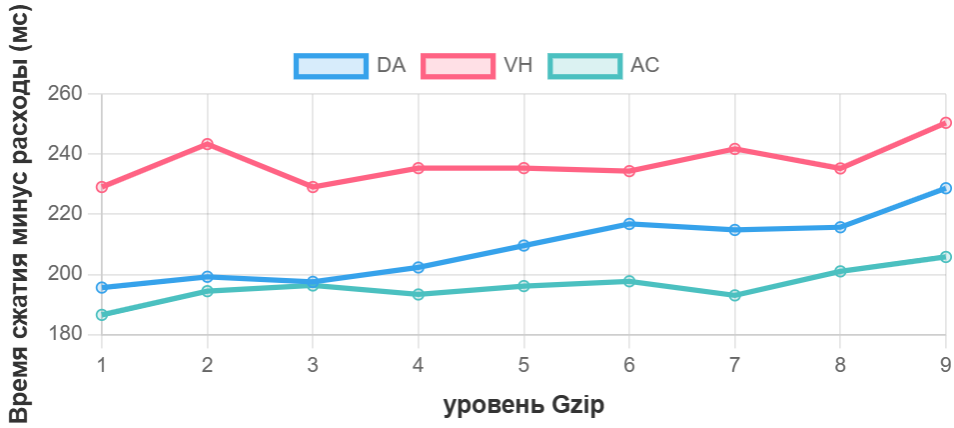
\includegraphics[width=\linewidth]{../images/Gzip compression time (min-overhead).png}
        \caption{Время сжатия Gzip за вычетом накладных расходов}
        \label{fig:image1}
    \end{minipage}
    \hfill
    \begin{minipage}{0.48\textwidth}
        \centering
        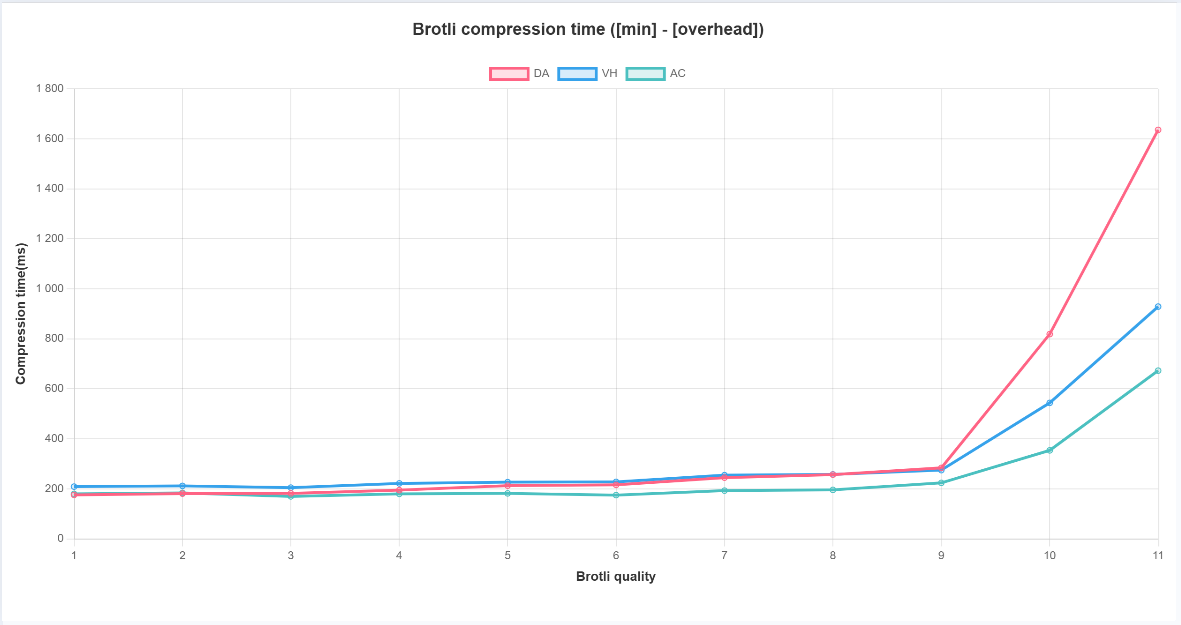
\includegraphics[width=\linewidth]{../images/Brotli compression time (min-overhead).png}
        \caption{Время сжатия Brotli за вычетом накладных расходов}
        \label{fig:image2}
    \end{minipage}
\end{figure}

Как можно заметить, время сжатия для Gzip почти не зависит от степени сжатия. Как следствие, можно пробовать сжимать динамические данные, применяя максимальный уровень.

У Brotli выделяются только два последних уровня — алгоритм тратит значительно больше времени. Для динамических данных лучше использовать уровни с 5-го по 9-й.

\subsubsection{Измерение времени декомпрессии}

Измерения времени декомпрессии программой gunzip произведены на Ubuntu Linux 24.04. Для замеров использована утилита hyperfine.

\begin{figure}[H]
    \centering
    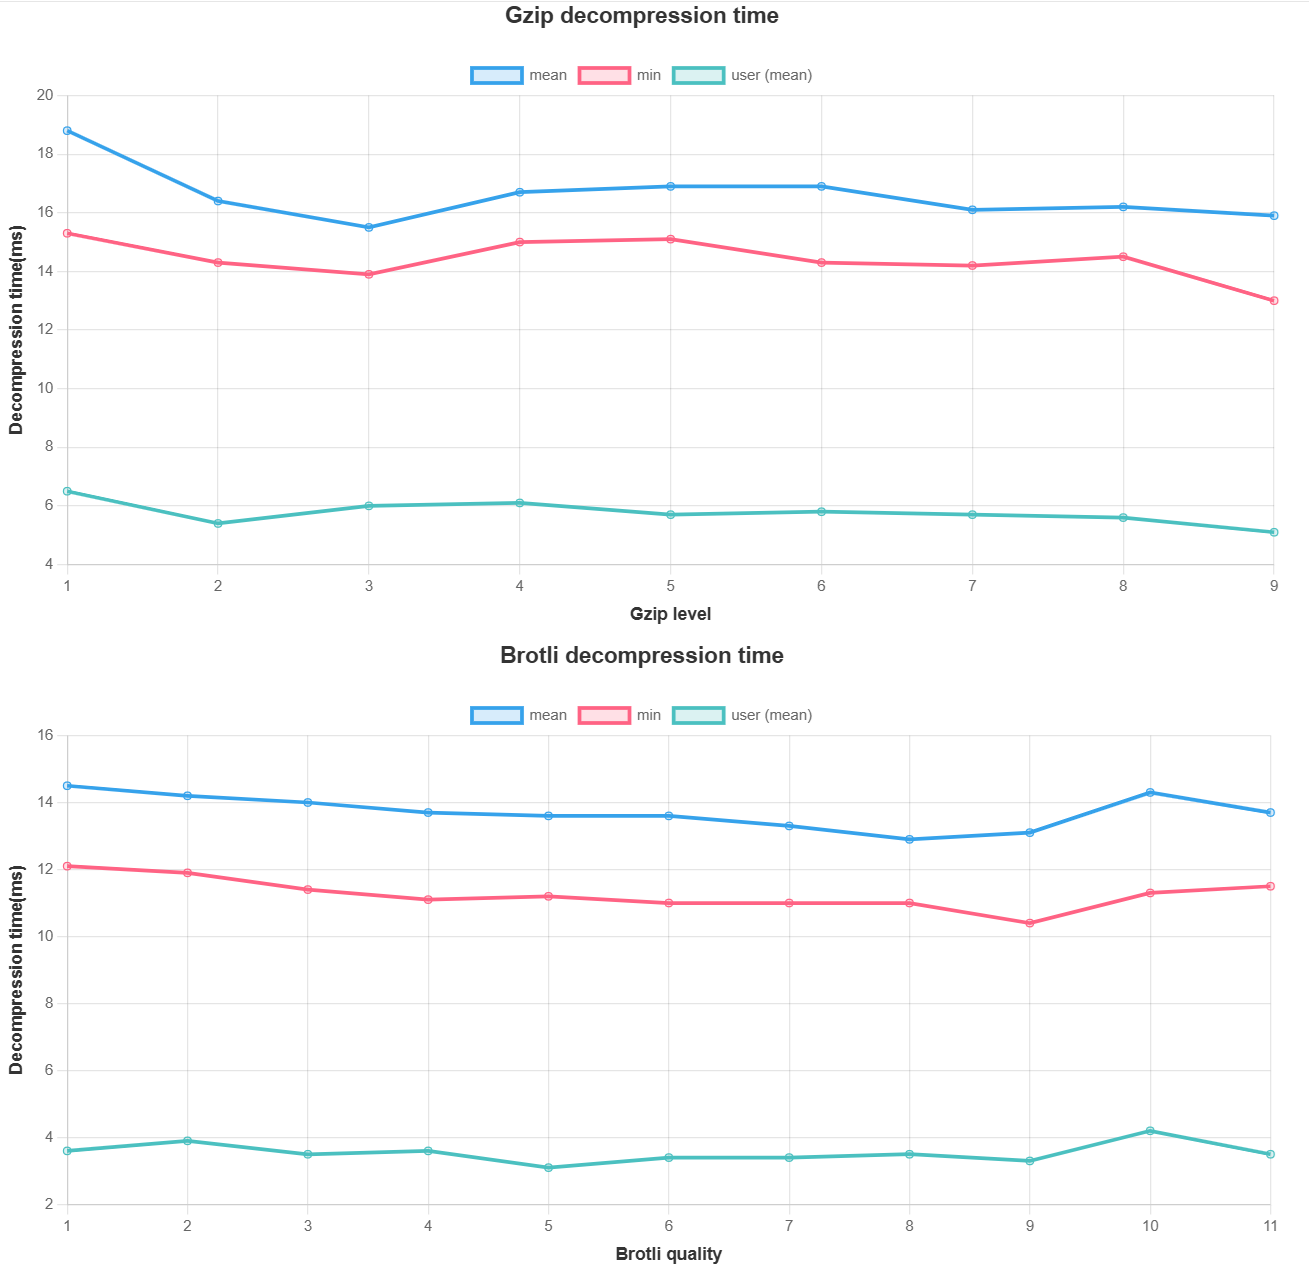
\includegraphics[width=1\textwidth]{../images/Decompression_time.png}
    \caption{Время декомпрессии Gzip и Brotli}
    \label{fig:decompression}
\end{figure}

Как видно из графика, скорость декомпрессии почти не зависит от степени сжатия. Это следует из асимметричности алгоритмов семейства LZ77.
Напрашивается вывод, что статические данные стоит сжимать максимально возможным образом.

Также стоит отметить, что Brotli в среднем быстрее разжимает файлы, чем Gzip (речь идёт о конкретных реализациях программ).

Итак, проанализировав результаты измерений, мы сделали выводы по практическому применению,
исходя из формулы (2). Посмотрим, к каким результатам мы придём, произведя замеры в консоли браузера для классического сценария работы пользователя.

\subsection{Реальные замеры сжатия статических файлов в браузере}

\subsubsection{Постановка эксперимента}

Смоделируем ситуацию, когда пользователь заходит на сайт и для продолжения работы ему нужно загрузить статические файлы (JS, CSS).

Для этого напишем следующий index.html:

\begin{lstlisting}[language=HTML]
<body>
    <script src="http://localhost:88/main.js" />
    <script>
        fetch("http://localhost:88/test");
    </script>
</body>
\end{lstlisting}

Принцип работы:
\begin{enumerate}
    \item Загружаем HTML-документ
    \item Парсим HTML-документ
    \item Встречаем тег \verb|<script src="http://localhost:88/main.js" />|,
          что означает необходимость загрузить и выполнить скрипт с указанного адреса.
          Дальнейшая обработка страницы приостанавливается до завершения загрузки и выполнения скрипта.
          В это время учитывается время, необходимое на скачивание и декодирование.
          Скрипт был закомментирован, чтобы не искажать измерения сторонними вычислениями.
    \item Выполняем запрос на "http://localhost:88/test". Этот запрос служит маркером. Время его отправки и будет измеряться.
\end{enumerate}

Будем измерять время отправки запроса для сжатия Brotli 11x и для файла без сжатия. Теоретически возможно, что вариант без сжатия окажется быстрее, так как не требует времени на декодирование.

Учитывая предположение, что CPU throttling не влияет на время декодирования, дополнительные замеры были проведены на мобильном телефоне Xiaomi 9T PRO в локальной Wi-Fi сети (300 Мбит/с).

Дополнительно было отключено кеширование на стороне клиента с помощью заголовков "Cache-Control" и "Pragma".

Как и в предыдущих экспериментах, были ограничены фоновые процессы. Для каждой конфигурации выполнено по 20 замеров.

В случае с телефоном время test-запроса измерялось на стороне сервера.

\begin{itemize}
    \item $T_{gzip9} = 65{,}35$ мс, $\sigma = 9{,}21$ мс
    \item $T_{no\_compress} = 145{,}10$ мс, $\sigma = 34{,}34$ мс
\end{itemize}

\subsubsection{Вывод по статическим файлам JS, CSS, HTML}

Результаты измерений показали, что для статических файлов сжатие во всех случаях либо существенно уменьшает время отклика, либо не увеличивает его.

Таким образом, для любых устройств и любых параметров сети сжатие статических файлов является предпочтительным. При этом следует выбирать максимальную степень сжатия — будь то gzip 9 или brotli 11.

\subsection{Нагрузочное тестирование REST-запросов (динамические данные)}

На данном этапе мы разобрались со статическими файлами. Теперь перейдём к динамическим данным, которые меняются с течением времени.
Основное отличие состоит в том, что мы не можем сжать данные заранее — приходится применять сжатие "на лету".
Наша задача — выяснить, как сжатие влияет на такие показатели, как:

\begin{itemize}
    \item количество запросов в секунду (RPS);
    \item нагрузку на сеть;
    \item время ожидания ответа от сервера;
    \item время загрузки содержимого запроса;
    \item общее время выполнения запроса.
\end{itemize}

\subsubsection{Описание аппаратной части сервера}

Технические характеристики сервера:
\begin{itemize}
    \item CPU: 1 vCPU;
    \item RAM: 2 ГБ;
    \item Storage: 20 ГБ;
    \item Скорость загрузки/отдачи: 1200 Мбит/с.
\end{itemize}

Технические характеристики ноутбука:
\begin{itemize}
    \item CPU: 4 ядра;
    \item RAM: 8 ГБ;
    \item Скорость загрузки/отдачи: 50 Мбит/с.
\end{itemize}

В качестве REST-сервера используется Node.js express.js, обратный прокси-сервер (сжатие HTTP) — Nginx.

Логика работы:
\begin{enumerate}
    \item Клиент заходит на сайт;
    \item Скачивает статические файлы;
    \item После выполнения JS-кода выполняется GET-запрос на получение всех видео (/videos/getAll);
    \item Сервер делает запрос в базу данных;
    \item Возвращает ответ.
\end{enumerate}

Тестирование проводится с помощью k6. Замеряются следующие параметры:
\begin{itemize}
    \item загрузка ЦП сервера;
    \item использование оперативной памяти сервера;
    \item время ожидания ответа от сервера;
    \item время загрузки содержимого запроса;
    \item процент успешно выполненных HTTP-запросов.
\end{itemize}

Тестирование проводится при разном количестве запросов в секунду (RPS).

Ответ от сервера представляет собой массив JSON:
\begin{lstlisting}[language=JavaScript]
[
  {
    title: "Steel Horizon",
    description: 
      '"Steel Horizon" is a captivating cinematic journey that explores the boundaries of imagination and reality. 
      With stunning visuals and a compelling narrative, it draws viewers into a richly woven tale full of emotion, suspense, 
      and intrigue. As the characters navigate through complex challenges, deep personal struggles, 
      and unexpected twists, the story unfolds with intensity and grace. Crafted by visionary creators, 
      the film blends elements of classic storytelling with modern cinematic techniques to create an unforgettable experience. 
      Whether you\'re drawn to heartfelt drama, thrilling action, or thought-provoking ideas, 
      this film offers a powerful reflection on humanity, resilience, and discovery.',
    number: 19,
    src_url: "https://cdn.example.com/videos/video_19.mp4",
    preview_url: "/previews/bearwolf.mp4",
    image_url: "/images/bearwolf2.jpg",
    studios: ["MegaPix"],
    tags: ["documentary", "action", "comedy"]
  }
]
\end{lstlisting}

\subsubsection{Физический смысл выбранной нагрузки}

\begin{figure}[H]
    \centering
    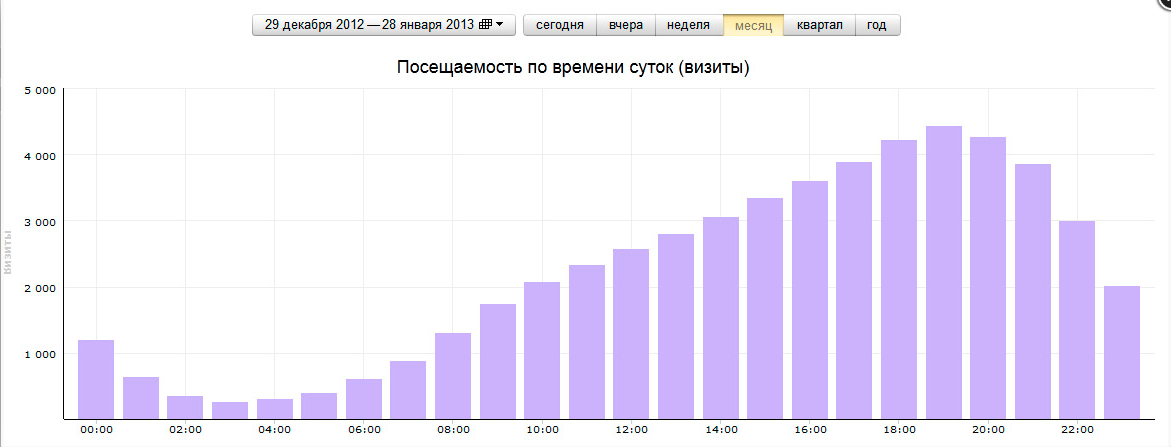
\includegraphics[width=1\textwidth]{../images/pedsovet.png}
    \caption{Количество посещений в час}
\end{figure}

Перед вами статистика посещаемости некоторого сайта за день. Собрано количество посещений за каждый час и построена гистограмма.
Можно заметить неравномерность визитов в течение дня: в период с 18:00 до 19:00 количество посещений составило около 4000,
а с 2:00 до 3:00 — менее 500. Это связано с территориальной распределённостью пользователей.

Если сайт русскоязычный, то логично предположить, что пик будет приходиться на вечернее время по Москве,
так как население России преимущественно находится в её европейской части. Поэтому важно понять, как ведёт себя сервер при разной нагрузке.

Было проведено два эксперимента, соответствующие пиковой и умеренной нагрузке.
Предполагается, что в условиях средне-низкой нагрузки, когда у ЦП есть достаточно ресурсов, сжатие проявит себя лучше, чем в условиях нехватки мощностей.

\subsubsection{Эксперимент первый}

Нагрузка:

\begin{lstlisting}[language=JavaScript]
  stages: [
    { duration: "5s", target: 10 },
    { duration: "10s", target: 20 },
    { duration: "10s", target: 30 },
    { duration: "10s", target: 40 },
    { duration: "10s", target: 50 },
    { duration: "10s", target: 60 },
    { duration: "10s", target: 70 },
    { duration: "10s", target: 80 },
    { duration: "10s", target: 90 },
    { duration: "10s", target: 100 },
    { duration: "10s", target: 110 },
    { duration: "10s", target: 120 },
    { duration: "10s", target: 130 },
    { duration: "10s", target: 140 },
    { duration: "10s", target: 150 },
    { duration: "10s", target: 170 },
    { duration: "10s", target: 190 },
    { duration: "10s", target: 210 },
    { duration: "5s", target: 5 },
  ]
\end{lstlisting}

duration - время каждой стадии, target - кол-во одновременно активных пользователей
Каждый пользователь отправляет запрос на сервер, ждёт ответа, далее ждёт 1 секунду и отправляет запрос снова.

\begin{table}[h]
    \centering
    \caption{Результаты без сжатия}
    \begin{tabular}{lr}
        \toprule
        \textbf{Метрика}                          & \textbf{Значение}               \\
        \midrule
        Всего проверок (checks\_total)            & 4662                            \\
        \hline
        Среднее время получения (receiving\_time) & \SI{2660}{\milli\second}        \\
        Минимальное время получения               & \SI{187}{\milli\second}         \\
        Медианное время получения                 & \SI{2388}{\milli\second}        \\
        Максимальное время получения              & \SI{45987}{\milli\second}       \\
        \hline
        Среднее общее время (total\_duration)     & \SI{2770}{\milli\second}        \\
        Медианное общее время                     & \SI{2492}{\milli\second}        \\
        90-й персентиль общего времени            & \SI{5476}{\milli\second}        \\
        \hline
        Среднее время ожидания (waiting\_time)    & \SI{106}{\milli\second}         \\
        \hline
        Средняя продолжительность HTTP-запроса    & \SI{2.7}{\second}               \\
        90-й персентиль HTTP-запросов             & \SI{5.47}{\second}              \\
        \hline
        Получено данных (Network data received)   & \SI{4.9}{\mega\byte\per\second} \\
        \bottomrule
    \end{tabular}
\end{table}

\begin{table}[h]
    \centering
    \caption{Результаты без сжатия}
    \begin{tabular}{lS[table-format=5.5]}
        \toprule
        \textbf{Метрика} & \textbf{Время (\si{\milli\second})} \\
        \midrule
        P50 (медиана)    & 2388                                \\
        P90              & 5320                                \\
        P95              & 6528                                \\
        Максимум         & 46186                               \\
        \bottomrule
    \end{tabular}
\end{table}

\begin{table}[h]
    \centering
    \caption{Результаты с сжатием (gzip 9)}
    \begin{tabular}{lr}
        \toprule
        \textbf{Метрика}                          & \textbf{Значение}               \\
        \midrule
        Всего проверок (checks\_total)            & 10324                           \\
        Частота проверок                          & \SI{57.0}{\per\second}          \\
        \hline
        Среднее время получения (receiving\_time) & \SI{1.45}{\milli\second}        \\
        Минимальное время получения               & \SI{6}{\milli\second}           \\
        Медианное время получения                 & \SI{1.00}{\milli\second}        \\
        Максимальное время получения              & \SI{592}{\milli\second}         \\
        \hline
        Среднее общее время (total\_duration)     & \SI{671}{\milli\second}         \\
        Медианное общее время                     & \SI{609}{\milli\second}         \\
        90-й персентиль общего времени            & \SI{1511}{\milli\second}        \\
        \hline
        Среднее время ожидания (waiting\_time)    & \SI{670}{\milli\second}         \\
        \hline
        Средняя продолжительность HTTP-запроса    & \SI{671}{\milli\second}         \\
        90-й персентиль HTTP-запросов             & \SI{1515}{\milli\second}        \\
        \hline
        Получено данных (Network data received)   & \SI{339}{\kilo\byte\per\second} \\
        \bottomrule
    \end{tabular}
\end{table}

\begin{table}[H]
    \centering
    \caption{Результаты с сжатием (gzip 9)}
    \begin{tabular}{lS[table-format=4.5]}
        \toprule
        \textbf{Метрика} & \textbf{Время (\si{\milli\second})} \\
        \midrule
        P50 (медиана)    & 609                                 \\
        P90              & 1511                                \\
        P95              & 1721                                \\
        Максимум         & 1958                                \\
        \bottomrule
    \end{tabular}
\end{table}

\subsubsection{Эксперимент второй}

Нагрузка:

\begin{lstlisting}[language=JavaScript]
   stages: [
    { duration: "10s", target: 10 },
    { duration: "20s", target: 10 },
    { duration: "20s", target: 15 },
    { duration: "20s", target: 20 },
    { duration: "20s", target: 25 },
    { duration: "20s", target: 30 },
    { duration: "10s", target: 5 },
  ]
\end{lstlisting}

\begin{table}[h]
    \centering
    \caption{Метрики производительности (без сжатия, эксперимент 2)}
    \label{tab:metrics}
    \begin{tabular}{lS[table-format=4.3]}
        \toprule
        \textbf{Метрика}                          & \textbf{Значение}               \\
        \midrule
        \multicolumn{2}{l}{\textbf{Основные показатели}}                            \\
        Всего проверок (checks\_total)            & 1454                            \\
        Частота проверок                          & \SI{12.0}{\per\second}          \\
        Скорость получения данных                 & \SI{2.5}{\mega\byte\per\second} \\
        \hline
        \multicolumn{2}{l}{\textbf{Временные характеристики}}                       \\
        Среднее время получения (receiving\_time) & 309.4\ мс                       \\
        Медианное время получения                 & 266.4\ мс                       \\
        Максимальное время получения              & 1099.2\ мс                      \\
        \hline
        Среднее общее время (total\_duration)     & 380.0\ мс                       \\
        Медианное общее время                     & 338.6\ мс                       \\
        90-й персентиль общего времени            & 518.7\ мс                       \\
        \hline
        Среднее время ожидания (waiting\_time)    & 70.5\ мс                        \\
        Медианное время ожидания                  & 69.4\ мс                        \\
        \hline
        Среднее время HTTP-запроса                & 380.0\ мс                       \\
        90-й персентиль HTTP-запросов             & 518.7\ мс                       \\
        \bottomrule
    \end{tabular}
\end{table}

\begin{table}[h]
    \centering
    \caption{Метрики производительности (gzip-9, эксперимент 2)}
    \begin{tabular}{lS[table-format=3.3]}
        \toprule
        \textbf{Метрика}                          & \textbf{Значение}              \\
        \midrule
        \multicolumn{2}{l}{\textbf{Основные показатели}}                           \\
        Всего проверок (checks\_total)            & 1861                           \\
        Частота проверок                          & \SI{15.4}{\per\second}         \\
        Скорость получения данных                 & \SI{92}{\kilo\byte\per\second} \\
        \hline
        \multicolumn{2}{l}{\textbf{Временные характеристики (мс)}}                 \\
        Среднее время получения (receiving\_time) & 1.77                           \\
        Медианное время получения                 & 1.72                           \\
        Максимальное время получения              & 65.9                           \\
        \hline
        Среднее общее время (total\_duration)     & 75.3                           \\
        Медианное общее время                     & 74.4                           \\
        90-й персентиль общего времени            & 81.0                           \\
        \hline
        Среднее время ожидания (waiting\_time)    & 73.4                           \\
        Медианное время ожидания                  & 72.6                           \\
        \hline
        Среднее время HTTP-запроса                & 75.3                           \\
        90-й персентиль HTTP-запросов             & 81.0                           \\
        \bottomrule
    \end{tabular}
\end{table}

\subsubsection{Анализ полученных результатов }

В первом эксперименте с пиковой нагрузкой прирост в количестве обработанных запросов составил 121\%, во втором - 28\%.
Заметим, что с ростом числа пользователей, несмотря на чудовищные по меркам сайтов $T_{req}=2,6$c,
сервер не отклоняет запросы, а ставит их в очередь. Максимальная длина очереди - число пользователей.
Пусть $V_{max}$ - максимальное число запросов, которое сервер может обработать в секунду.
Найдём $T_{req}$ в \textbf{установившемся пиковом} режиме.
Условие установившегося режима - количество поступающих запросов совпадает с количеством обработанных:

\[
    \frac{N_{users}}{T_{req} + T_{wait}}=V_{\text{max}}
\]

\[
    T_{req} = \frac{N_{users}}{V_{\text{max}}} - T_{wait}
\]

Из этой формулы можно найти максимальное число пользователей, при котором начнут отклоняться http запросы:

\begin{equation}
    N^{\text{крит}}_{users} = (T^{\text{крит}}_{req} + T_{wait}){V_{\text{max}}}
\end{equation}

Так, для $T^{\text{крит}}_{req} = 10$с, $T_{wait}=1$c, $V_{max}=80$RPS, $N^{\text{крит}}_{users}=880$

В первом эксперименте обе конфигурации вышли на пиковый режим. В случае без сжатия узким горлышком оказалась сеть, во втором - мощность процессора.

\subsubsection{Зависимость CPU load, Network load от уровня сжатия}

Ограничение на скорость создано искусственно с помощью настройки роутера QoS, максимальная скорость около 200 Mb/s\\
Ограничие скорости гарантирует постоянную полосу пропускания\\
На сервере отключены все построронние процессы. CPU используется только для:

\begin{itemize}
    \item MySQL Database
    \item Backend server (Express.js)
    \item Обратный прокси сервер (Nginx)
\end{itemize}

Нагрузка:

\begin{lstlisting}[language=JavaScript]
  stages: [
    { duration: "5s", target: 10 },
    { duration: "10s", target: 20 },
    { duration: "10s", target: 30 },
    { duration: "10s", target: 40 },
    { duration: "10s", target: 50 },
    { duration: "10s", target: 60 },
    { duration: "10s", target: 70 },
    { duration: "10s", target: 80 },
    { duration: "10s", target: 90 },
    { duration: "10s", target: 100 },
    { duration: "10s", target: 110 },
    { duration: "10s", target: 120 },
    { duration: "10s", target: 130 },
    { duration: "10s", target: 140 },
    { duration: "10s", target: 150 },
    { duration: "10s", target: 170 },
    { duration: "10s", target: 190 },
    { duration: "10s", target: 210 },
    { duration: "5s", target: 5 },
  ]
\end{lstlisting}

В базе данных находится 400 видео, для тестирования используется Get запрос:
\verb|/video/getRecomendations/1|, который возвращает 100 случайных видео из базы данных. Около 100 видео, нужно для реализации корректного
скроллинга. (В одной строке можно разместить 5 видео, На экране помещается 5 строк, хотим закрыть
потребность в 3 скролах без подзагрузки, получаем 100 видео).

Будет варироваться степень сжатия:
\begin{itemize}
    \item no compress
    \item gzip 1
    \item gzip 5
    \item gzip 9
\end{itemize}

При построении графиков использовалось сглаживание по трём точкам

\[
    x^{smooth}_{i} = \frac{x_{i-1} + x_{i} + x_{i+1}}{3}
\]

Построены графики от времени

Результаты измерений:

\begin{table}[h]
    \centering
    \caption{Метрики производительности (без сжатия)}
    \begin{tabular}{lr}
        \toprule
        \textbf{Метрика}                       & \textbf{Значение}               \\
        \midrule
        Общее время теста                      & 3 минуты 01 секунда             \\
        \hline
        Всего проверок (checks\_total)         & 11827                           \\
        Частота проверок                       & \SI{65.3}{\per\second}          \\
        \hline
        Средняя продолжительность HTTP-запроса & \SI{456.3}{\milli\second}       \\
        Минимальное время ответа               & \SI{134.3}{\milli\second}       \\
        Медианное время ответа                 & \SI{232.7}{\milli\second}       \\
        Максимальное время ответа              & \SI{1.67}{\second}              \\
        90-й персентиль                        & \SI{1.13}{\second}              \\
        95-й персентиль                        & \SI{1.28}{\second}              \\
        \hline
        Объём полученных данных                & \SI{1.2}{\giga\byte}            \\
        Скорость получения данных              & \SI{6.9}{\mega\byte\per\second} \\
        \bottomrule
    \end{tabular}
\end{table}

\begin{table}[h]
    \centering
    \caption{Метрики производительности (gzip сжатие уровень 1)}
    \begin{tabular}{lr}
        \toprule
        \textbf{Метрика}                       & \textbf{Значение}               \\
        \midrule
        Общее время теста                      & 3 минуты                        \\
        \hline
        Всего проверок (checks\_total)         & 12745                           \\
        Частота проверок                       & \SI{70.3}{\per\second}          \\
        \hline
        Средняя продолжительность HTTP-запроса & \SI{350}{\milli\second}         \\
        Минимальное время ответа               & \SI{47.5}{\milli\second}        \\
        Медианное время ответа                 & \SI{146.1}{\milli\second}       \\
        Максимальное время ответа              & \SI{1.27}{\second}              \\
        90-й персентиль                        & \SI{994.4}{\milli\second}       \\
        95-й персентиль                        & \SI{1.07}{\second}              \\
        \hline
        Объём полученных данных                & \SI{57}{\mega\byte}             \\
        Скорость получения данных              & \SI{316}{\kilo\byte\per\second} \\
        \bottomrule
    \end{tabular}
\end{table}

\begin{table}[h]
    \centering
    \caption{Метрики производительности (gzip сжатие уровень 5)}
    \begin{tabular}{lr}
        \toprule
        \textbf{Метрика}                       & \textbf{Значение}               \\
        \midrule
        Общее время теста                      & 3 минуты                        \\
        \hline
        Всего проверок (checks\_total)         & 12338                           \\
        Частота проверок                       & \SI{68.1}{\per\second}          \\
        \hline
        Средняя продолжительность HTTP-запроса & \SI{396}{\milli\second}         \\
        Минимальное время ответа               & \SI{47.7}{\milli\second}        \\
        Медианное время ответа                 & \SI{157}{\milli\second}         \\
        Максимальное время ответа              & \SI{1.57}{\second}              \\
        99-й персентиль                        & \SI{1.05}{\second}              \\
        95-й персентиль                        & \SI{1.21}{\second}              \\
        \hline
        Объём полученных данных                & \SI{48}{\mega\byte}             \\
        Скорость получения данных              & \SI{266}{\kilo\byte\per\second} \\
        \bottomrule
    \end{tabular}
\end{table}

\begin{table}[h]
    \centering
    \caption{Метрики производительности (gzip сжатие уровень 9)}
    \begin{tabular}{lr}
        \toprule
        \textbf{Метрика}               & \textbf{Значение}               \\
        \midrule
        Общее время теста              & 3 минуты 01 секунда             \\
        \hline
        Всего проверок (checks\_total) & 12214                           \\
        Частота запросов               & \SI{67.4}{\per\second}          \\
        \hline
        Среднее время HTTP-запроса     & \SI{411.3}{\milli\second}       \\
        Минимальное время ответа       & \SI{44.3}{\milli\second}        \\
        Медианное время ответа         & \SI{338}{\milli\second}         \\
        Максимальное время ответа      & \SI{1.52}{\second}              \\
        90-й персентиль                & \SI{1.12}{\second}              \\
        95-й персентиль                & \SI{1.23}{\second}              \\
        \hline
        Объём полученных данных        & \SI{45}{\mega\byte}             \\
        Скорость передачи данных       & \SI{248}{\kilo\byte\per\second} \\
        \bottomrule
    \end{tabular}
\end{table}

\begin{figure}[H]
    \centering
    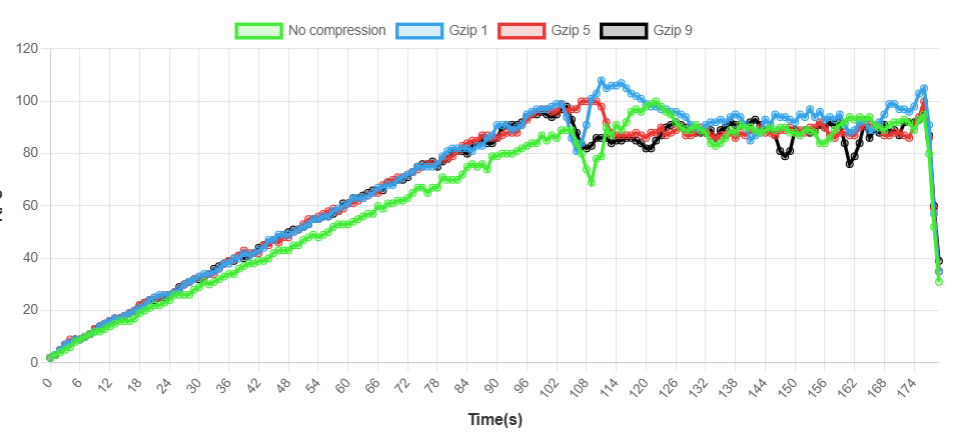
\includegraphics[width=1\textwidth]{../images/second_part/RPS.png}
    \caption{Количество запросов в секунду}
\end{figure}

\begin{figure}[H]
    \centering
    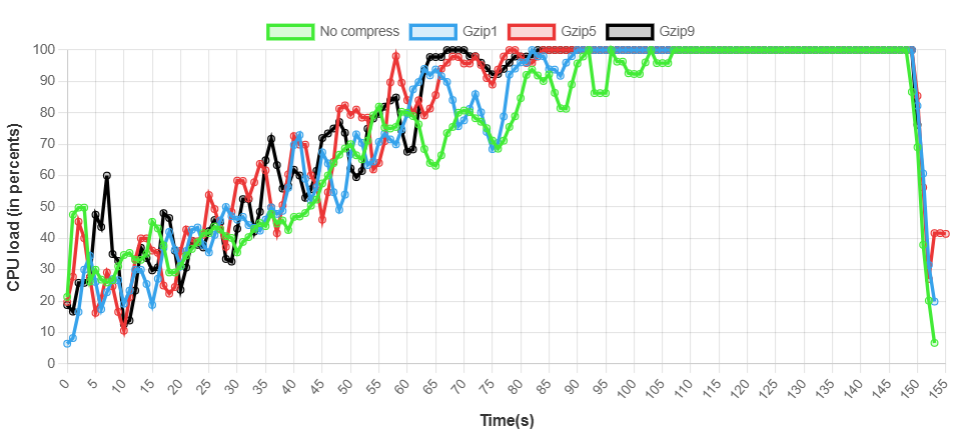
\includegraphics[width=1\textwidth]{../images/second_part/CPU_load.png}
    \caption{Загрузка CPU}
\end{figure}

\begin{figure}[H]
    \centering
    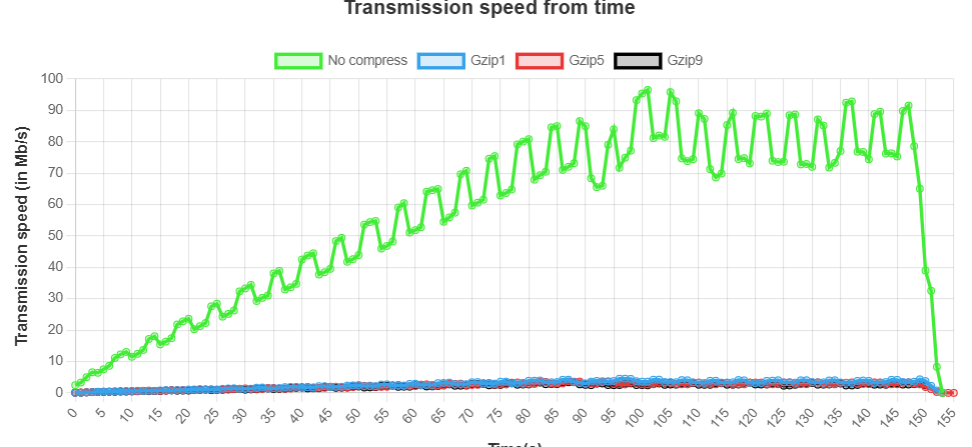
\includegraphics[width=1\textwidth]{../images/second_part/Transmission_speed.png}
    \caption{Загрузка сети}
\end{figure}

\begin{figure}[H]
    \centering
    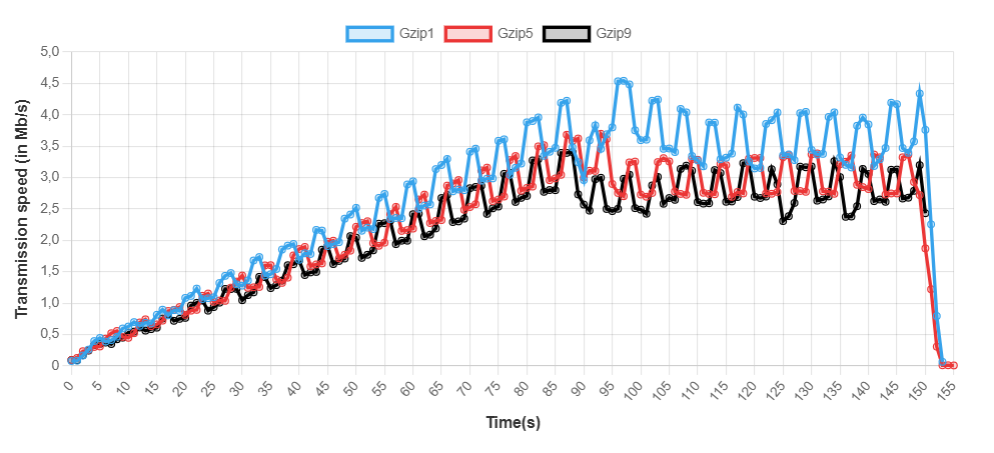
\includegraphics[width=1\textwidth]{../images/second_part/Transmission_speed_withot_nocompress.png}
    \caption{Загрузка сети только для сжатых запросов}
\end{figure}

\subsubsection{Анализ полученных результатов}

Нетрудно заметить, что использовние gzip заментно снизило нагрузку на сеть примерно в 20-30 раз,
при этом даже при 80 МБ/c несжатого трафика, нагрузка на CPU из-за сжатия оказалась крайне малой, что при загрузке CPU на 100\%,
показатель RPS остался на том же уровне.

Теперь выведем математические соотношения для нашей схемы эксперимента, из которых найдём оптимальные параметры сжатия.
Оптимальными будем считать такие параметры, при которых достигается максимум RPS.

\[
    V_{RPS} = V_{RPS}(N_{users}, i_{comp})
\]

где $N_{users}$ - количество активных пользователей, выполняющих запросы. $i_{comp}$ - уровень (качество, в случае Brotli) сжатия.

Рассмотрим сначала случай, когда у сервера всего один поток. Пусть на сервер пришёл один HTTP запрос, очередь пуста. Сервер последовательно выполнит следующие шаги:

\begin{enumerate}
    \item Принять HTTP запрос, аутентифицировать пользователя
    \item Сделать запрос в базу данных и подобрать персональные рекомендации,
    \item Применить сжатие к телу HTTP ответа
    \item Отправитть ответ пользователю
\end{enumerate}

В случае, если пользователей много, могут образовываться очереди. Одна очередь связана с обработкой ответа, вторая с загрузкой тела запроса.

\begin{figure}[H]
    \centering
    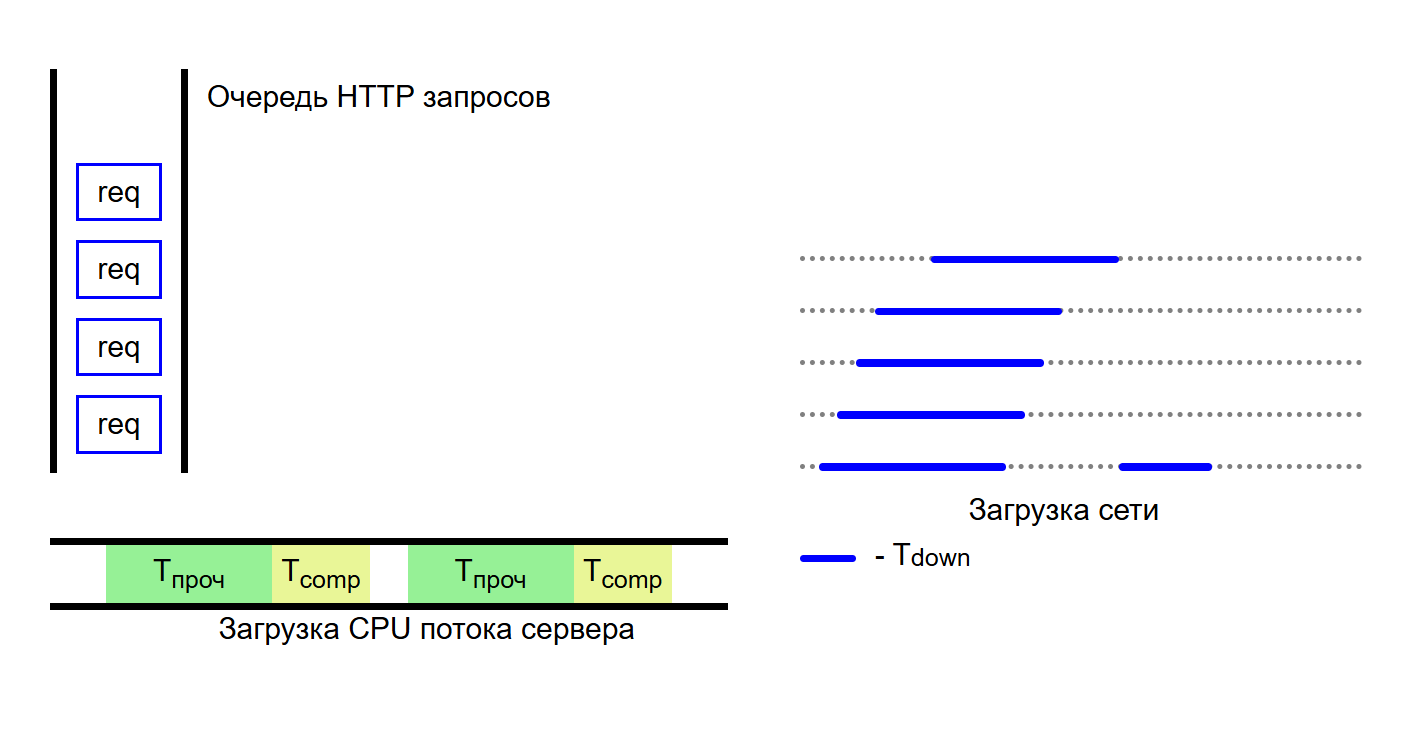
\includegraphics[width=1\textwidth]{../images/timing-model.png}
    \caption{Временная модель сервера}
\end{figure}

Если в данный момент в установившемся режиме $N \gg 1$ активных пользователей, можно ввести следующие характеристики:

\begin{itemize}
    \item $\overline{Q}_{HTTP}$ - среднее по времени число пользователей в очереди HTTP запросов,
    \item $\overline{Q}_{down}$ - среднее по времени число пользователей в очереди на скачивание,
\end{itemize}

RPS вычисляется по формуле:

\[
    RPS = \frac{N}{\overline{T}_{\text{полн}}}
\]

где $\overline{T}_{\text{полн}}$ - среднее полное время одного запроса:

Для конкретного запроса $T_{\text{полн}}$ рассчитывается по формуле:

\begin{equation}
    T_{\text{полн}} = T_{ping} + T_{\text{handle}}*(1 + Q_{HTTP}) + T_{down} + T_{decomp} + T_{wait}
\end{equation}

где:

\begin{itemize}
    \item $T_{ping}$ - время на сетевые задержки, связанные с удалённостью сервера и сетевым оборудования,
    \item $T_{\text{handle}} = T_{\text{проч} + T_{\text{сomp}}}$ - время на обработку одного запроса. В него входит время на аутентификацию, запрос к базе данных, сжатия тела HTTP ответа,
    \item $T_{wait}$ - фиксированная пауза для каждого пользователя,

\end{itemize}

Считая $T_{decom}$ пренебрежительно малым (ассиметричность алгоритмов LZ77):

\[
    T_{\text{полн}} = T_{ping} + T_{\text{handle}}*(1 + Q_{HTTP}) + T_{down}
\]

$T_{down}$ вычисляется по формуле:

\[
    T_{down} = \frac{M_{\text{исх}}*(Q_{down} + 1)}{k_{i}*V_{min}}
\]

где:

\begin{itemize}
    \item $M_{\text{исх}}$ - исходный размер тела HTTP ответа в байтах,
    \item $k_{i}$ - степень сжатия $i-\text{го}$ уровня,
    \item $V_{min}$ - минимум из скорости отдачи backend сервера и скорости загрузки нагрузочного сервера
\end{itemize}

Получаем:

\[
    T_{\text{полн}} = T_{ping} + T_{\text{handle}}*(1 + Q_{HTTP}) + \frac{M_{\text{исх}}*(Q_{down} + 1)}{k_{i}*V_{min}} + T_{wait}
\]

Предположим, что увеличилось число пользователей. Тогда начнут увеличиваться длины очередей, увеличится полное время запросов
и RPS останется прежним. Таким образом достигается бесперебойная работа сервера.

Разумно предположить, что вероятность нахождение пользователей в очереди равно отношению среднего времени, проведённого в очереди
, к среднему полному времени запроса. Тогда:

\begin{equation}
    \overline{Q}_{HTTP} = P_{HTTP} * N = \frac{T_{\text{handle}} * (\overline{Q}_{HTTP} + 1)}{T_{\text{полн}}} * N
\end{equation}

\begin{equation}
    \overline{Q}_{down} = P_{down} * N = \frac{M_{\text{исх}}*(\overline{Q}_{down} + 1)}{k_{i}*V_{min}} * \frac{1}{T_{\text{полн}}} * N = \frac{M_{\text{исх}}*(\overline{Q}_{down} + 1)}{T_{\text{полн}} * k_{i}*V_{min}} * N
\end{equation}

\begin{spacing}{2.0}
    Проверим формулу (5) в простых случаях. Пусть $T_{handle} \ll T_{\text{полн}}$, тогда правая часть равна нулю, $\overline{Q}_{HTTP} = 0$.
    Введём $\alpha_{HTTP} = \frac{T_{handle} * N}{T_{full}}$, $0 \le \alpha{HTTP} \le \frac{N}{1+N}$, тогда $\overline{Q}_{HTTP} = \frac{\alpha_{HTTP}}{1 - \alpha_{HTTP}}$.
    Если $\overline{Q}_{HTTP} = N$, то есть все в очереди на обработку запроса,
    то $T_{\text{полн}} = T_{handle}*(N+1) \approx T_{handle}*N$, при  $N \gg 1$
\end{spacing}

Обозначим $\alpha_{down} = \frac{М_{\text{исх}} * N}{T_{\text{полн}}*k_{i}*V_{min}}$ и подставив в (4),
усреднив по времени, найдём $T_{\text{полн}}$ через число пользователей и уровень сжатия:

\begin{equation}
    T_{\text{полн}} = T_{ping} + T_{wait} + T_{handle}*\frac{1}{1 - \alpha_{HTTP}} + \frac{M_{\text{исх}}}{k_{i}*V_{min}} * \frac{1}{1 - \alpha_{down}}
\end{equation}

Применим полученную формулу для объяснения результатов экспериментов. Для начала покажем, что $RPS$ достигнет порогового значения в случае использования Gzip.

Частью, отвечающей за скачивание, можно пренебречь, т.к она меньше на два порядка времени ожидания ответа от сервера. Тогда:

\[
    T_{\text{полн}} = T_{ping} + T_{wait} + T_{handle}*\frac{1}{1 - \alpha_{HTTP}}
\]

Решая численно уравнение, построим график $RPS$ от $N$

\begin{figure}[H]
    \centering
    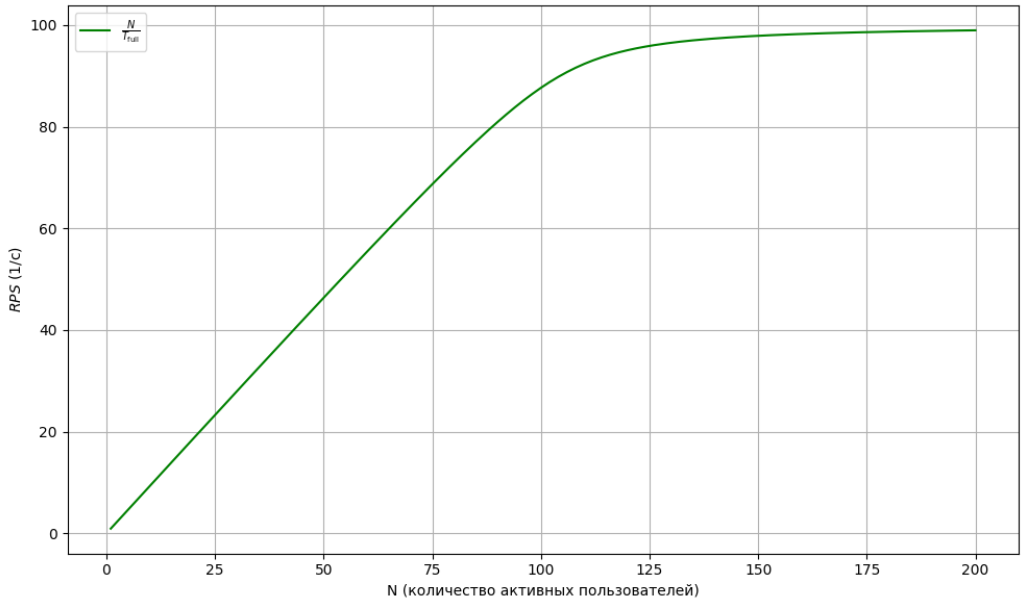
\includegraphics[width=1\textwidth]{../images/rps-from-n.png}
    \caption{Зависимость $RPS$ от $N$}
\end{figure}

При построении графика использованы следующие значения:

\begin{itemize}
    \item $T_{ping} = 60   \text{ мс}$
    \item $T_{wait} = 1000 \text{ мс}$
    \item $T_{handle} = 10 \text{ мс}$
\end{itemize}

Итак мы получили формулу, связывающую $RPS$ и степень сжатия. Перебором можно найти максимальный $RPS$. В этом заключается смысл алгоритма переключателя.

\subsection{Реализация переключателя}

Чтобы реализовать переключатель степени сжатия, используя указанный стек технологий, можно использовать один из 3-х способов:

\subsubsection{Дополнительный обратный прокси сервер на Express.js}

При первой попытке создания переключателя стало понятно, что стандартная реализация библиотеки Gzip и в целом Nginx не поддерживают динамическое изменение степени сжатия для конкретного HTTP запроса. То есть в Nginx можно прописать разное сжатие по адресам, это выглядит примерно так:

\begin{lstlisting}[
    basicstyle=\ttfamily\small,
    keywordstyle=\color{blue},
    commentstyle=\color{black},
    stringstyle=\color{red},
    numbers=left,
    numberstyle=\tiny\color{gray},
    frame=single,
    breaklines=true,
    backgroundcolor=\color{white}
]
http {
    gzip on;
    gzip_types application/json text/plain text/css application/javascript application/xml;
    gzip_min_length 100;
    gzip_vary on;
    include /etc/nginx/conf.d/*.conf;

    server {
        listen 3002;
        add_header Vary Accept-Encoding;

        location ^~ /gzip/1/ {
            gzip_comp_level 1;
            rewrite ^/gzip/1/(.*)$ /$1 break;
            proxy_pass http://server:3001;
        }

        location ^~ /gzip/2/ {
            gzip_comp_level 2;
            rewrite ^/gzip/2/(.*)$ /$1 break;
            proxy_pass http://server:3001;
        }
    }
}
\end{lstlisting}

То есть для адреса `/gzip/1/*` применяем сжатие gzip 1, для адреса `/gzip/2/*` применем сжатие gzip 2 и т.д. Но браузер сам не будет получать информацию о загрузке сети и процессора сервера и перенаправлять запросы. Для этой задачи я использовал ещё один обратный прокси сервер на Express js, который проверял с заданным промежутком загрузку процессора и перенаправлял запрос `/someadress/` на `/gzip/n/someadress`.

К сожалению, затраты на создание ещё одного прокси оказались слишком велики, при любой конфигурации сети,
количество обработанных запросов такого переключателя было более чем на 10\% меньше чем статическое сжатие с помощью Nginx gzip 1.

\subsubsection{Реконфигуратор Nginx }

Существует команда `nginx -s reload`, которая выполняет безопасную перезагрузку конфигурационного файла

Получив сигнал, главный процесс проверяет правильность синтаксиса нового конфигурационного файла и пытается применить содержащуюся в нём конфигурацию:
\begin{itemize}
    \item Если это удаётся, главный процесс запускает новые рабочие процессы и отправляет сообщения старым рабочим процессам с требованием завершиться.
    \item В противном случае главный процесс откатывает изменения и продолжает работать со старой конфигурацией.
\end{itemize}

Старые рабочие процессы, получив команду завершиться, прекращают принимать новые запросы и продолжают обслуживать текущие запросы, пока все такие запросы не будут обслужены. После этого старые рабочие процессы завершаются.

Таким образом, эта команда позволяет в реальном времени без опасения потерять необработанные запросы сменить конфигурационный файл. Было создано 10 конфигурационных файлов: 1 без сжатия, 9 - для каждого уровня gzip. И с помощью дополнительной
программы менял их и перезагружал Nginx

\subsubsection{Модуль для Nginx}

Для Nginx можно написать свой модуль, который будет выполнять роль переключателя. В ходе данной работы я его не реализовал

\section{Общие выводы}

В ходе работы мы рассмотрели применение методов сжатия на примере реального веб-приложения для оптимизации таких ключевых метрик, как LCP и RPS.
Проведён сравнительный анализ с точки зрения степени сжатия, времени компрессии/декопрессии. Построена модель backend сервера,
найдены зависимости между нагрузкой на сеть и на ЦП. Построена модель для оценки времени запроса от сервера.
Были получены условия на выбор оптимальных параметров сжатия и на их основе даны практические рекомендации.
Реализовано и предложено несколько вариантов переключателя, используя уже существующий стек технологий.

Стоит отметить, что в случае моего сервера, переключатель не потребовался. Вне зависимости от числа пользователей,
накладные расходы на сжатие полностью окупились бенефитами от снижения нагрузки на сеть.

\subsection{План дальнейших исследований}

Хотелось бы провести замеры на крупном проекте с высоким трафиком. Применить теорию массового обслуживания для установления более точных
соотношений между метриками. Реализовать модуль для Nginx, чтобы снизить накладные расходы на переключатель.

\begin{thebibliography}{9}
    \bibitem{rfc1950}
    P. Deutsch, J. Gailly,
    \textit{RFC 1950: ZLIB Compressed Data Format Specification},
    IETF, May 1996.
    \url{https://tools.ietf.org/html/rfc1950}

    \bibitem{rfc1951}
    P. Deutsch,
    \textit{RFC 1951: DEFLATE Compressed Data Format Specification},
    IETF, May 1996.
    \url{https://tools.ietf.org/html/rfc1951}

    \bibitem{rfc1952}
    P. Deutsch,
    \textit{RFC 1952: GZIP File Format Specification},
    IETF, May 1996.
    \url{https://tools.ietf.org/html/rfc1952}

    \bibitem{brotli}
    L. Zhelyazkov et al.,
    \textit{RFC 7932: Brotli Compressed Data Format},
    IETF, July 2016.
    \url{https://tools.ietf.org/html/rfc7932}

    \bibitem{rfc2616}
    R. Fielding et al.,
    \textit{RFC 2616: Hypertext Transfer Protocol -- HTTP/1.1},
    IETF, June 1999 (Section 3.5: Content Codings).
    \url{https://tools.ietf.org/html/rfc2616#section-3.5}

    \bibitem{compression-book}
    Ватолин Д., Ратушняк А., Смирнов М., Юкин В.,
    \textit{Методы сжатия данных. Устройство архиваторов, сжатие изображений и видео},
    М.: ДИАЛОГ-МИФИ, 2002, с. 75--116.

    \bibitem{data-compression}
    D. Salomon, G. Motta,
    \textit{Handbook of Data Compression},
    5th ed., Springer, 2010.

    \bibitem{express}
    Express.js Documentation,
    \textit{Express - Node.js web application framework},
    \url{https://expressjs.com/}

    \bibitem{react}
    React Documentation,
    \textit{React - A JavaScript library for building user interfaces},
    \url{https://reactjs.org/docs/getting-started.html}

    \bibitem{node}
    Node.js Documentation,
    \textit{Node.js JavaScript Runtime},
    \url{https://nodejs.org/en/docs/}

    \bibitem{k6}
    k6 Documentation,
    \textit{k6 - Open-source load testing tool},
    \url{https://k6.io/docs/}

    \bibitem{nginx}
    NGINX Documentation,
    \textit{NGINX - High Performance Load Balancer, Web Server \& Reverse Proxy},
    \url{https://nginx.org/en/docs/}

    \bibitem{compression-algorithms}
    M. Nelson, J. Gailly,
    \textit{The Data Compression Book},
    2nd ed., M\&T Books, 1995.

    \bibitem{modern-compression}
    I.H. Witten et al.,
    \textit{Managing Gigabytes: Compressing and Indexing Documents and Images},
    Morgan Kaufmann, 1999.
\end{thebibliography}
\end{document}